
%% bare_jrnl.tex
%% V1.4
%% 2012/12/27
%% by Michael Shell
%% see http://www.michaelshell.org/
%% for current contact information.
%%
%% This is a skeleton file demonstrating the use of IEEEtran.cls
%% (requires IEEEtran.cls version 1.8 or later) with an IEEE journal paper.
%%
%% Support sites:
%% http://www.michaelshell.org/tex/ieeetran/
%% http://www.ctan.org/tex-archive/macros/latex/contrib/IEEEtran/
%% and
%% http://www.ieee.org/



% *** Authors should verify (and, if needed, correct) their LaTeX system  ***
% *** with the testflow diagnostic prior to trusting their LaTeX platform ***
% *** with production work. IEEE's font choices can trigger bugs that do  ***
% *** not appear when using other class files.                            ***
% The testflow support page is at:
% http://www.michaelshell.org/tex/testflow/


%%*************************************************************************
%% Legal Notice:
%% This code is offered as-is without any warranty either expressed or
%% implied; without even the implied warranty of MERCHANTABILITY or
%% FITNESS FOR A PARTICULAR PURPOSE!
%% User assumes all risk.
%% In no event shall IEEE or any contributor to this code be liable for
%% any damages or losses, including, but not limited to, incidental,
%% consequential, or any other damages, resulting from the use or misuse
%% of any information contained here.
%%
%% All comments are the opinions of their respective authors and are not
%% necessarily endorsed by the IEEE.
%%
%% This work is distributed under the LaTeX Project Public License (LPPL)
%% ( http://www.latex-project.org/ ) version 1.3, and may be freely used,
%% distributed and modified. A copy of the LPPL, version 1.3, is included
%% in the base LaTeX documentation of all distributions of LaTeX released
%% 2003/12/01 or later.
%% Retain all contribution notices and credits.
%% ** Modified files should be clearly indicated as such, including  **
%% ** renaming them and changing author support contact information. **
%%
%% File list of work: IEEEtran.cls, IEEEtran_HOWTO.pdf, bare_adv.tex,
%%                    bare_conf.tex, bare_jrnl.tex, bare_jrnl_compsoc.tex,
%%                    bare_jrnl_transmag.tex
%%*************************************************************************

% Note that the a4paper option is mainly intended so that authors in
% countries using A4 can easily print to A4 and see how their papers will
% look in print - the typesetting of the document will not typically be
% affected with changes in paper size (but the bottom and side margins will).
% Use the testflow package mentioned above to verify correct handling of
% both paper sizes by the user's LaTeX system.
%
% Also note that the "draftcls" or "draftclsnofoot", not "draft", option
% should be used if it is desired that the figures are to be displayed in
% draft mode.
%
\documentclass[journal]{IEEEtran}
%
% If IEEEtran.cls has not been installed into the LaTeX system files,
% manually specify the path to it like:
% \documentclass[journal]{../sty/IEEEtran}





% Some very useful LaTeX packages include:
% (uncomment the ones you want to load)


% *** MISC UTILITY PACKAGES ***
%
%\usepackage{ifpdf}
% Heiko Oberdiek's ifpdf.sty is very useful if you need conditional
% compilation based on whether the output is pdf or dvi.
% usage:
% \ifpdf
%   % pdf code
% \else
%   % dvi code
% \fi
% The latest version of ifpdf.sty can be obtained from:
% http://www.ctan.org/tex-archive/macros/latex/contrib/oberdiek/
% Also, note that IEEEtran.cls V1.7 and later provides a builtin
% \ifCLASSINFOpdf conditional that works the same way.
% When switching from latex to pdflatex and vice-versa, the compiler may
% have to be run twice to clear warning/error messages.






% *** CITATION PACKAGES ***
%
\usepackage{cite}
% cite.sty was written by Donald Arseneau
% V1.6 and later of IEEEtran pre-defines the format of the cite.sty package
% \cite{} output to follow that of IEEE. Loading the cite package will
% result in citation numbers being automatically sorted and properly
% "compressed/ranged". e.g., [1], [9], [2], [7], [5], [6] without using
% cite.sty will become [1], [2], [5]--[7], [9] using cite.sty. cite.sty's
% \cite will automatically add leading space, if needed. Use cite.sty's
% noadjust option (cite.sty V3.8 and later) if you want to turn this off
% such as if a citation ever needs to be enclosed in parenthesis.
% cite.sty is already installed on most LaTeX systems. Be sure and use
% version 4.0 (2003-05-27) and later if using hyperref.sty. cite.sty does
% not currently provide for hyperlinked citations.
% The latest version can be obtained at:
% http://www.ctan.org/tex-archive/macros/latex/contrib/cite/
% The documentation is contained in the cite.sty file itself.






% *** GRAPHICS RELATED PACKAGES ***
%
\ifCLASSINFOpdf
   \usepackage[pdftex]{graphicx}
  % declare the path(s) where your graphic files are
  % \graphicspath{{../pdf/}{../jpeg/}}
  % and their extensions so you won't have to specify these with
  % every instance of \includegraphics
    \DeclareGraphicsExtensions{.pdf,.jpeg,.png}
\else
  % or other class option (dvipsone, dvipdf, if not using dvips). graphicx
  % will default to the driver specified in the system graphics.cfg if no
  % driver is specified.
  % \usepackage[dvips]{graphicx}
  % declare the path(s) where your graphic files are
  % \graphicspath{{../eps/}}
  % and their extensions so you won't have to specify these with
  % every instance of \includegraphics
  % \DeclareGraphicsExtensions{.eps}
\fi
% graphicx was written by David Carlisle and Sebastian Rahtz. It is
% required if you want graphics, photos, etc. graphicx.sty is already
% installed on most LaTeX systems. The latest version and documentation
% can be obtained at:
% http://www.ctan.org/tex-archive/macros/latex/required/graphics/
% Another good source of documentation is "Using Imported Graphics in
% LaTeX2e" by Keith Reckdahl which can be found at:
% http://www.ctan.org/tex-archive/info/epslatex/
%
% latex, and pdflatex in dvi mode, support graphics in encapsulated
% postscript (.eps) format. pdflatex in pdf mode supports graphics
% in .pdf, .jpeg, .png and .mps (metapost) formats. Users should ensure
% that all non-photo figures use a vector format (.eps, .pdf, .mps) and
% not a bitmapped formats (.jpeg, .png). IEEE frowns on bitmapped formats
% which can result in "jaggedy"/blurry rendering of lines and letters as
% well as large increases in file sizes.
%
% You can find documentation about the pdfTeX application at:
% http://www.tug.org/applications/pdftex





% *** MATH PACKAGES ***
%
\usepackage[cmex10]{amsmath}
% A popular package from the American Mathematical Society that provides
% many useful and powerful commands for dealing with mathematics. If using
% it, be sure to load this package with the cmex10 option to ensure that
% only type 1 fonts will utilized at all point sizes. Without this option,
% it is possible that some math symbols, particularly those within
% footnotes, will be rendered in bitmap form which will result in a
% document that can not be IEEE Xplore compliant!
%
% Also, note that the amsmath package sets \interdisplaylinepenalty to 10000
% thus preventing page breaks from occurring within multiline equations. Use:
%\interdisplaylinepenalty=2500
% after loading amsmath to restore such page breaks as IEEEtran.cls normally
% does. amsmath.sty is already installed on most LaTeX systems. The latest
% version and documentation can be obtained at:
% http://www.ctan.org/tex-archive/macros/latex/required/amslatex/math/





% *** SPECIALIZED LIST PACKAGES ***
%
% \usepackage{algorithmicx}
\usepackage{algorithm}
%\usepackage{algorithmicx}
\usepackage{algpseudocode}
% algorithmic.sty was written by Peter Williams and Rogerio Brito.
% This package provides an algorithmic environment fo describing algorithms.
% You can use the algorithmic environment in-text or within a figure
% environment to provide for a floating algorithm. Do NOT use the algorithm
% floating environment provided by algorithm.sty (by the same authors) or
% algorithm2e.sty (by Christophe Fiorio) as IEEE does not use dedicated
% algorithm float types and packages that provide these will not provide
% correct IEEE style captions. The latest version and documentation of
% algorithmic.sty can be obtained at:
% http://www.ctan.org/tex-archive/macros/latex/contrib/algorithms/
% There is also a support site at:
% http://algorithms.berlios.de/index.html
% Also of interest may be the (relatively newer and more customizable)
% algorithmicx.sty package by Szasz Janos:
% http://www.ctan.org/tex-archive/macros/latex/contrib/algorithmicx/




% *** ALIGNMENT PACKAGES ***
%
%\usepackage{array}
% Frank Mittelbach's and David Carlisle's array.sty patches and improves
% the standard LaTeX2e array and tabular environments to provide better
% appearance and additional user controls. As the default LaTeX2e table
% generation code is lacking to the point of almost being broken with
% respect to the quality of the end results, all users are strongly
% advised to use an enhanced (at the very least that provided by array.sty)
% set of table tools. array.sty is already installed on most systems. The
% latest version and documentation can be obtained at:
% http://www.ctan.org/tex-archive/macros/latex/required/tools/


% IEEEtran contains the IEEEeqnarray family of commands that can be used to
% generate multiline equations as well as matrices, tables, etc., of high
% quality.




% *** SUBFIGURE PACKAGES ***
%\ifCLASSOPTIONcompsoc
%  \usepackage[caption=false,font=normalsize,labelfont=sf,textfont=sf]{subfig}
%\else
%  \usepackage[caption=false,font=footnotesize]{subfig}
%\fi
% subfig.sty, written by Steven Douglas Cochran, is the modern replacement
% for subfigure.sty, the latter of which is no longer maintained and is
% incompatible with some LaTeX packages including fixltx2e. However,
% subfig.sty requires and automatically loads Axel Sommerfeldt's caption.sty
% which will override IEEEtran.cls' handling of captions and this will result
% in non-IEEE style figure/table captions. To prevent this problem, be sure
% and invoke subfig.sty's "caption=false" package option (available since
% subfig.sty version 1.3, 2005/06/28) as this is will preserve IEEEtran.cls
% handling of captions.
% Note that the Computer Society format requires a larger sans serif font
% than the serif footnote size font used in traditional IEEE formatting
% and thus the need to invoke different subfig.sty package options depending
% on whether compsoc mode has been enabled.
%
% The latest version and documentation of subfig.sty can be obtained at:
% http://www.ctan.org/tex-archive/macros/latex/contrib/subfig/




% *** FLOAT PACKAGES ***
%
%\usepackage{fixltx2e}
% fixltx2e, the successor to the earlier fix2col.sty, was written by
% Frank Mittelbach and David Carlisle. This package corrects a few problems
% in the LaTeX2e kernel, the most notable of which is that in current
% LaTeX2e releases, the ordering of single and double column floats is not
% guaranteed to be preserved. Thus, an unpatched LaTeX2e can allow a
% single column figure to be placed prior to an earlier double column
% figure. The latest version and documentation can be found at:
% http://www.ctan.org/tex-archive/macros/latex/base/


%\usepackage{stfloats}
% stfloats.sty was written by Sigitas Tolusis. This package gives LaTeX2e
% the ability to do double column floats at the bottom of the page as well
% as the top. (e.g., "\begin{figure*}[!b]" is not normally possible in
% LaTeX2e). It also provides a command:
%\fnbelowfloat
% to enable the placement of footnotes below bottom floats (the standard
% LaTeX2e kernel puts them above bottom floats). This is an invasive package
% which rewrites many portions of the LaTeX2e float routines. It may not work
% with other packages that modify the LaTeX2e float routines. The latest
% version and documentation can be obtained at:
% http://www.ctan.org/tex-archive/macros/latex/contrib/sttools/
% Do not use the stfloats baselinefloat ability as IEEE does not allow
% \baselineskip to stretch. Authors submitting work to the IEEE should note
% that IEEE rarely uses double column equations and that authors should try
% to avoid such use. Do not be tempted to use the cuted.sty or midfloat.sty
% packages (also by Sigitas Tolusis) as IEEE does not format its papers in
% such ways.
% Do not attempt to use stfloats with fixltx2e as they are incompatible.
% Instead, use Morten Hogholm'a dblfloatfix which combines the features
% of both fixltx2e and stfloats:
%
% \usepackage{dblfloatfix}
% The latest version can be found at:
% http://www.ctan.org/tex-archive/macros/latex/contrib/dblfloatfix/




%\ifCLASSOPTIONcaptionsoff
%  \usepackage[nomarkers]{endfloat}
% \let\MYoriglatexcaption\caption
% \renewcommand{\caption}[2][\relax]{\MYoriglatexcaption[#2]{#2}}
%\fi
% endfloat.sty was written by James Darrell McCauley, Jeff Goldberg and
% Axel Sommerfeldt. This package may be useful when used in conjunction with
% IEEEtran.cls'  captionsoff option. Some IEEE journals/societies require that
% submissions have lists of figures/tables at the end of the paper and that
% figures/tables without any captions are placed on a page by themselves at
% the end of the document. If needed, the draftcls IEEEtran class option or
% \CLASSINPUTbaselinestretch interface can be used to increase the line
% spacing as well. Be sure and use the nomarkers option of endfloat to
% prevent endfloat from "marking" where the figures would have been placed
% in the text. The two hack lines of code above are a slight modification of
% that suggested by in the endfloat docs (section 8.4.1) to ensure that
% the full captions always appear in the list of figures/tables - even if
% the user used the short optional argument of \caption[]{}.
% IEEE papers do not typically make use of \caption[]'s optional argument,
% so this should not be an issue. A similar trick can be used to disable
% captions of packages such as subfig.sty that lack options to turn off
% the subcaptions:
% For subfig.sty:
% \let\MYorigsubfloat\subfloat
% \renewcommand{\subfloat}[2][\relax]{\MYorigsubfloat[]{#2}}
% However, the above trick will not work if both optional arguments of
% the \subfloat command are used. Furthermore, there needs to be a
% description of each subfigure *somewhere* and endfloat does not add
% subfigure captions to its list of figures. Thus, the best approach is to
% avoid the use of subfigure captions (many IEEE journals avoid them anyway)
% and instead reference/explain all the subfigures within the main caption.
% The latest version of endfloat.sty and its documentation can obtained at:
% http://www.ctan.org/tex-archive/macros/latex/contrib/endfloat/
%
% The IEEEtran \ifCLASSOPTIONcaptionsoff conditional can also be used
% later in the document, say, to conditionally put the References on a
% page by themselves.




% *** PDF, URL AND HYPERLINK PACKAGES ***
%
%\usepackage{url}
% url.sty was written by Donald Arseneau. It provides better support for
% handling and breaking URLs. url.sty is already installed on most LaTeX
% systems. The latest version and documentation can be obtained at:
% http://www.ctan.org/tex-archive/macros/latex/contrib/url/
% Basically, \url{my_url_here}.




% *** Do not adjust lengths that control margins, column widths, etc. ***
% *** Do not use packages that alter fonts (such as pslatex).         ***
% There should be no need to do such things with IEEEtran.cls V1.6 and later.
% (Unless specifically asked to do so by the journal or conference you plan
% to submit to, of course. )


% correct bad hyphenation here
\hyphenation{op-tical net-works semi-conduc-tor}


\begin{document}
%
% paper title
% can use linebreaks \\ within to get better formatting as desired
% Do not put math or special symbols in the title.
\title{Inside Coronary Arteries from X-ray Angiograms}
%
%
% author names and IEEE memberships
% note positions of commas and nonbreaking spaces ( ~ ) LaTeX will not break
% a structure at a ~ so this keeps an author's name from being broken across
% two lines.
% use \thanks{} to gain access to the first footnote area
% a separate \thanks must be used for each paragraph as LaTeX2e's \thanks
% was not built to handle multiple paragraphs
%

\author{Xinglong Liu, Fei Hou$^*$, Aimin Hao, Hong Qin
\thanks{Xinglong Liu, Fei Hou and Aimin Hao are at the State Key Laboratory of Virtual Reality Technology and Systems, Beihang University.}%
\thanks{Hong Qin is at the Department of Computer Science, Stony Brook University.}%
\thanks{$^*$Corresponding author, email: houfei@vrlab.buaa.edu.cn}}

% note the % following the last \IEEEmembership and also \thanks -
% these prevent an unwanted space from occurring between the last author name
% and the end of the author line. i.e., if you had this:
%
% \author{....lastname \thanks{...} \thanks{...} }
%                     ^------------^------------^----Do not want these spaces!
%
% a space would be appended to the last name and could cause every name on that
% line to be shifted left slightly. This is one of those "LaTeX things". For
% instance, "\textbf{A} \textbf{B}" will typeset as "A B" not "AB". To get
% "AB" then you have to do: "\textbf{A}\textbf{B}"
% \thanks is no different in this regard, so shield the last } of each \thanks
% that ends a line with a % and do not let a space in before the next \thanks.
% Spaces after \IEEEmembership other than the last one are OK (and needed) as
% you are supposed to have spaces between the names. For what it is worth,
% this is a minor point as most people would not even notice if the said evil
% space somehow managed to creep in.



% The paper headers
%\markboth{Journal of \LaTeX\ Class Files,~Vol.~11, No.~4, December~2012}%
%{Shell \MakeLowercase{\textit{et al.}}: Bare Demo of IEEEtran.cls for Journals}
% The only time the second header will appear is for the odd numbered pages
% after the title page when using the twoside option.
%
% *** Note that you probably will NOT want to include the author's ***
% *** name in the headers of peer review papers.                   ***
% You can use \ifCLASSOPTIONpeerreview for conditional compilation here if
% you desire.




% If you want to put a publisher's ID mark on the page you can do it like
% this:
%\IEEEpubid{0000--0000/00\$00.00~\copyright~2012 IEEE}
% Remember, if you use this you must call \IEEEpubidadjcol in the second
% column for its text to clear the IEEEpubid mark.



% use for special paper notices
%\IEEEspecialpapernotice{(Invited Paper)}




% make the title area
\maketitle

% As a general rule, do not put math, special symbols or citations
% in the abstract or keywords.
\begin{abstract}
In this paper, we present a labeling method for coronary arteries from X-ray angiogram based on energy optimization. The fundamental goal is to assist the analysis and diagnosis of interventional surgery in the most efficient ways. We also hope our method can improve the performance during doctor training, surgery simulation and planning. We start with a fully parallelized algorithm based on Hessian Matrix to extract the tubular structures from the X-ray angiogram as vessel candidates. Then, instead of using the candidates directly, we use the Grow Cut method which is similar with Graph Cut but with better performance to extract the precise vessel structures from the images. Next, we use the Fast Marching method with second derivatives and cross neighbors to extract accurate skeleton segments. After that, we proposed a method based on Iterative Closet Point(ICP) to organize skeleton segments with the consideration of continuity and similarity. Finally, we formulate the vessel labeling problem into an energy optimization problem and solve it using belief propagation. Several typical applications including flow velocity estimation, heart beat estimation and vessel diameter estimation using our method have been given to show its practical use in clinical diagnosis and treatment. We envision that our system would be of high assistance for diagnosis and therapy to treat vessel-related diseases in a clinical setting in the near future.
\end{abstract}

% Note that keywords are not normally used for peerreview papers.
\begin{IEEEkeywords}
X-ray Angiograms, Coronary Artery, Energy Optimization
\end{IEEEkeywords}



% For peer review papers, you can put extra information on the cover
% page as needed:
% \ifCLASSOPTIONpeerreview
% \begin{center} \bfseries EDICS Category: 3-BBND \end{center}
% \fi
%
% For peerreview papers, this IEEEtran command inserts a page break and
% creates the second title. It will be ignored for other modes.
\IEEEpeerreviewmaketitle



\section{Introduction}
% The very first letter is a 2 line initial drop letter followed
% by the rest of the first word in caps.
%
% form to use if the first word consists of a single letter:
% \IEEEPARstart{A}{demo} file is ....
%
% form to use if you need the single drop letter followed by
% normal text (unknown if ever used by IEEE):
% \IEEEPARstart{A}{}demo file is ....
%
% Some journals put the first two words in caps:
% \IEEEPARstart{T}{his demo} file is ....
%
% Here we have the typical use of a "T" for an initial drop letter
% and "HIS" in caps to complete the first word.
\IEEEPARstart{T}{he} morbidity of Cardiovascular Disease(CVD) is rapidly increasing over the past few decades. The golden standard for diagnosis of CVD is X-ray coronary angiography. Reading and analyzing angiogram is a compulsory course for fresh physicians involved in intervention surgery or for diagnosis of heart disease. Even though the imaging techniques have been developing rapidly, leading to better performance and imaging quality, there are still shortcomings such as view angle dependance, overlapping and blurring, etc. Accurate coronary arteries segmentation and recognition is necessary for both cardiologist-in-training and medical practitioners towards diagnosis, surgery planning and treatment. This paper's originality hinges upon our novel solution to extract coronary arteries and recognize each artery with known labels. Besides, we apply our method in practical cases, digging the inside information from the X-ray angiograms which will give better guidance for later treatments.

Even though various work has been done to achieve better understanding of cardiovascular angiograms, there are still some unsolved challenges existing in current methods. First, the angiograms are with low contrast and high dynamic range and sometimes even blurry or incomplete. It is hard to extract the vessel structures from the images accurately. Second, current methods are time consuming while there are tons of angiograms produced daily from cardiologists, making it hard to process these valuable materials in time. Third, the skeleton organization step in current methods is based on either prior knowledge or geometrical structures and cannot ensure a globally optimized solution. At last, current methods calculate parameters of coronary arteries such as flow velocity just from pixels on the images without considering  the global vessel structures and the structure relationship between images, which is not only wasting the information from the images but also not accurate.

To overcome these shortcomings, we present an efficient vessel extraction and labeling method, as well as several applications using the proposed method including flow velocity estimation, heart beat rate estimation, etc. The pipeline is shown in Fig.~\ref{fig:pipeline} consisting four stages: vessel and skeleton extraction(Section~\ref{sec:vessel-skeleton-extraction}), vessel organization(Section~\ref{sec:vessel-organization}), tree structure labeling(Section~\ref{sec:tree-labeling}) and application(Section~\ref{sec:application}). In the first stage, we design a parallel algorithm based on Hessian Matrix~\cite{Frangi} to extract candidate vessels and Grow Cut method based on Cellar Automaton to further process the candidates for more accurate foreground coronary arteries and backgrounds. In the second stage, we propose an iterative distance and similarity evaluation method based on Iterative Closest Point(ICP) with global optimization nature to organize extracted vessel skeleton segments. After this stage, all vessel segments are organized as well structured trees. In the third stage, we formulate the labeling problem of the organized skeletons into an energy optimization problem and solve it using belief propagation. At last, in the fourth stage, we applied our method to several practical estimation problem to help for better diagnosis and treatment. The main contributions of our work include:
\begin{itemize}
\item An efficient parallelized vessel extraction and thinning method using both Hessian Matrix and Grow Cut method with the consideration of both the probability and the continuity of being vessels.

\item A novel iterative distance and similarity evaluation method based on ICP and the framework based on this descriptor to transform the extracted vessel skeletons into well structured trees.

\item A novel labeling method based on energy optimization solved using belief propagation with \textit{distance} and \textit{topology} constrains, which is robust to noisy and incomplete data from images.

\item Several typical practical applications using the proposed method to help for better understanding inside the X-ray angiograms.
\end{itemize}

\begin{figure*}[!t]
\centering
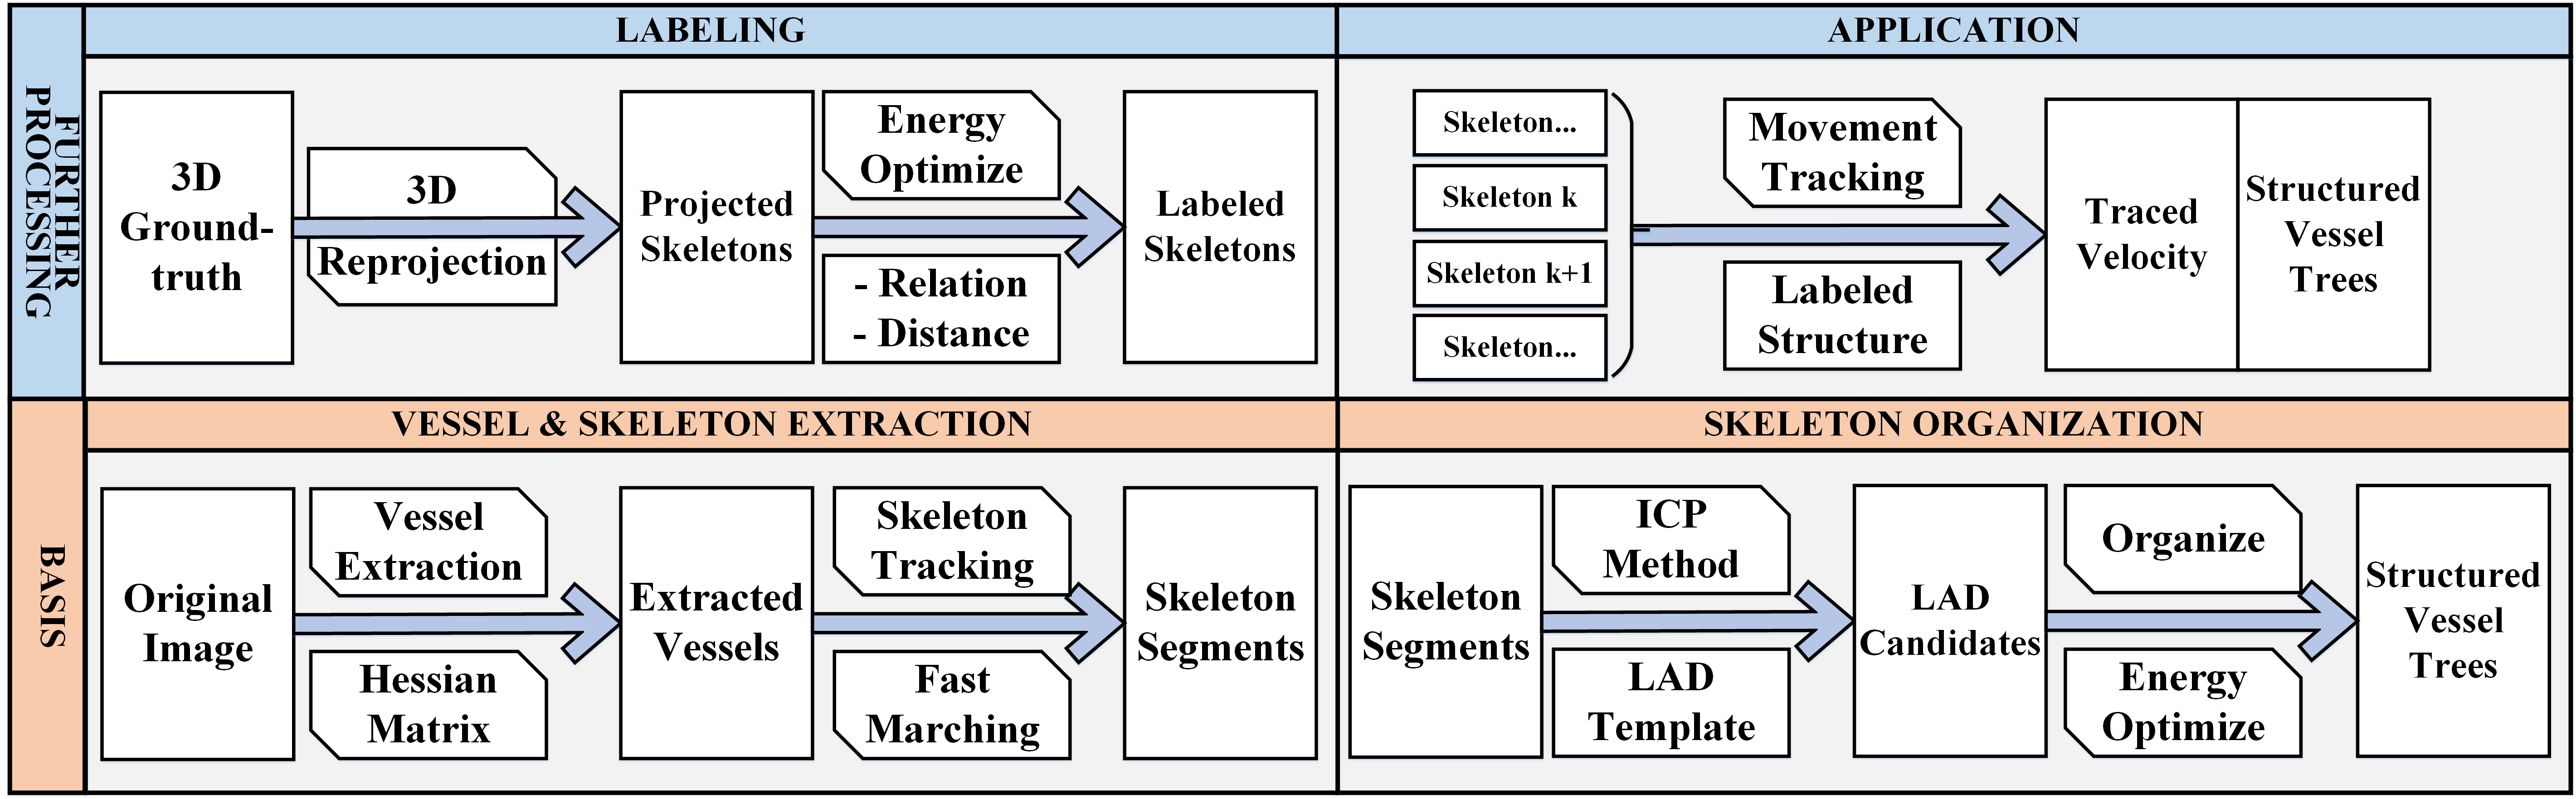
\includegraphics[width=1.0\linewidth]{./images/pipeline.png}
\caption{Work pipeline.}
\label{fig:pipeline}
\end{figure*}

%%%%%%%%%%%%%%%%%%%%%%%%%%%%%%%%%%%%%%%%%%%%
\section{Related Work}
\label{sec:related-work}
Our work relates to vessel extraction, skeleton tracking, energy optimization, etc. We now briefly review them in the following categories.

\subsection{Vessel Extraction}
According to the difference of starting point for each technique and thinking way, the vessel extraction methods can be divided into these categories: pattern recognition techniques (PR), deformable model based techniques~\cite{Deformable2}\cite{Deformable3}, tracking-based techniques~\cite{Tracking2}\cite{Tracking3}\cite{Tracking5}, artificial intelligence based techniques, neural network based techniques, and miscellaneous tube-like object detection techniques. Each one contains many sub-types such as multi-scale approaches, mathematical morphology approaches. Readers could refer to~\cite{Kirbas} for an overview. Besides, Hoover et al.~\cite{Hoover} used a mathematical filter to offer a broad range of vessel enhancement, and Li et al.~\cite{Li} conducted this task using a non-linear filter. Frangi et al.~\cite{Frangi} used the eigen values of Hessian matrix to extract the tube-like structures from X-ray images. Condurache et al.~\cite{Condurache} used this method while adding a hysteresis thresholding method to purify the extracted data. But they are not robust to handle blurry images. Zhang et al.~\cite{Zhang2010438} proposed a novel extension of the matched filter approach which is composed of a zero-mean Gaussian function and the first-order derivative of Gaussian, yet their extraction may lead to more isolated retinal vessels.

\subsection{Skeleton Extraction}
Typically, vessels extracted from angiograms are quite complicated.  Centerline extraction for vessels is essential for both data implication and further processing. Van et al.~\cite{van2007subvoxel} and Hassouna et al.~\cite{Hassouna2007} proposed methods based on Eikonal Equation and fast marching method to find vessel skeletons. Yet, they can not process isolated vessel segments. Zhang et al.~\cite{two_step_thinning} proposed a two step thinning method based on the structure analysis of the candidate vessel structures. Tracking based techniques are also popular in this area. Most thinning methods are hard to be parallelized.

\subsection{Vessel Labeling}
Subsection text here.

\subsection{Optimization Techniques}
Optimization techniques are widely used in various areas such as image restoration, 3D reconstruction, etc. Geman et al.~\cite{geman1984stochastic} first proposed the classical theories of Markov Random Field (MRF), Gibbs Sampling and Maximum a Posteriori estimate. Lafferty et al.~\cite{lafferty2001conditional} proposed the Conditional Random Field (CRF) which provides a tool for structural classification and prediction. Based on these theories, Belief Propagation (BP) was proposed by Pearl~\cite{pearl1982reverend} to solve the optimization problems in MRF. From then on, many applications have been done with the help with BP, including performance studies~\cite{Meltzer2005}~\cite{murphy1999loopy} ~\cite{szeliski2008comparative}~\cite{tappen2003comparison}, speedup methods~\cite{potetz2008efficient}~\cite{brunton2006belief} ~\cite{coughlan2007dynamic}~\cite{felzenszwalb2006efficient}, etc. Besides BP, Graph Cut (GC) is also an energy minimization method which is better in first-order MRF than BP, and much better than dynamic programming, gradient decedent, simulated annealing, etc. GC is widely used in computer vision including image segmentation~\cite{boykov2001interactive}, stereo disparity and motion~\cite{boykov2001fast}. In~\cite{boykov2001fast}, Boykov presented an efficient $\alpha$-expansion and $\alpha$-$\beta$ swap algorithm for metric energy minimization based on GC. Kolmogorov et al.~\cite{kolmogorov2004energy} introduced the characteristics of the energy function which could be minimized by GC and conducted the genetic construction of the minimization function. Based on graph cut, there are many extensions, such as Grow Cut~\cite{vezhnevets2005growcut}, Grab Cut~\cite{rother2004grabcut} et al. We formulate the labeling problem as a discrete energy optimization problem solved by BP.

\subsection{Practical Applications}
Several approaches have been proposed to extract the inside information including blood flow speed, vessel movements from the X-ray angiograms.

%%%%%%%%%%%%%%%%%%%%%%%%%%%%%%%%%%%%%%%%%%%%
\section{Vessel and Skeleton Extraction}
\label{sec:vessel-skeleton-extraction}
It is important to segment the vessels as well as skeletons from the raw data precisely, both as the basis for further processing and for data simplification. Given X-ray angiograms, we design an efficient algorithm with the help of GPU for extracting enhanced images as vessel candidates (Section.~\ref{subsubsec:hessian}). After that, we split the candidates into \textit{background}, \textit{foreground(vessels)} and \textit{undefined}. Then, Grow Cut method which is based on Cellar Automaton is used to select \textit{foreground} from \textit{undefined} with the knowledge from known \textit{foreground}, \textit{background} and vessel continuity (Section.~\ref{subsubsec:growcut}). At last, we apply the Multistencils Fast Marching method with second derivative and cross neighbors to track skeletons from segmented vessels (Section~\ref{subsec:skeleton-extraction}). The final segmented and skeletonized results are shown in Fig.~\ref{fig:step1_result}.

\begin{figure}[!t]
\centering
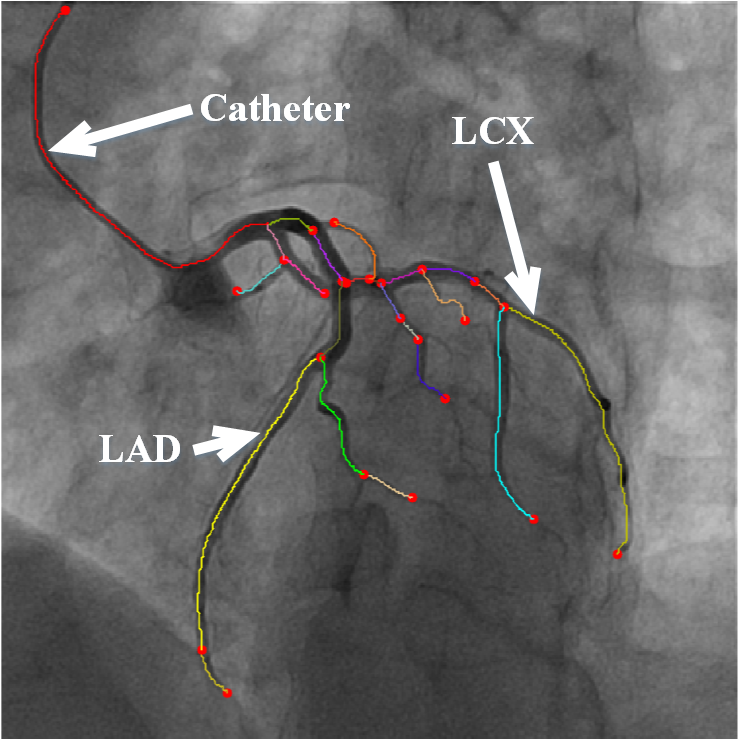
\includegraphics[width=1.0\linewidth]{./images/step1_result.png}
\caption{Results for vessel and skeleton extraction. Catheter, LAD and LCX branch are identified. Different colors correspond to different segments. Round filled circles are used to identify bifurcation and distal points.}
\label{fig:step1_result}
\end{figure}

\subsection{Vessel Extraction}
\label{subsec:vessel-extraction}
Original angiograms acquired from X-ray machines suffer from low contrast, high dynamic range and low lumen. To overcome these shortcomings, we use a global optimization method which consists of three parts including vessel enhancement, Hessian based vessel candidates extraction and Grow Cut based global optimized precise exact extraction. The pipeline is described in Fig.~\ref{fig:pip_extraction}.

\begin{figure}[!t]
\centering
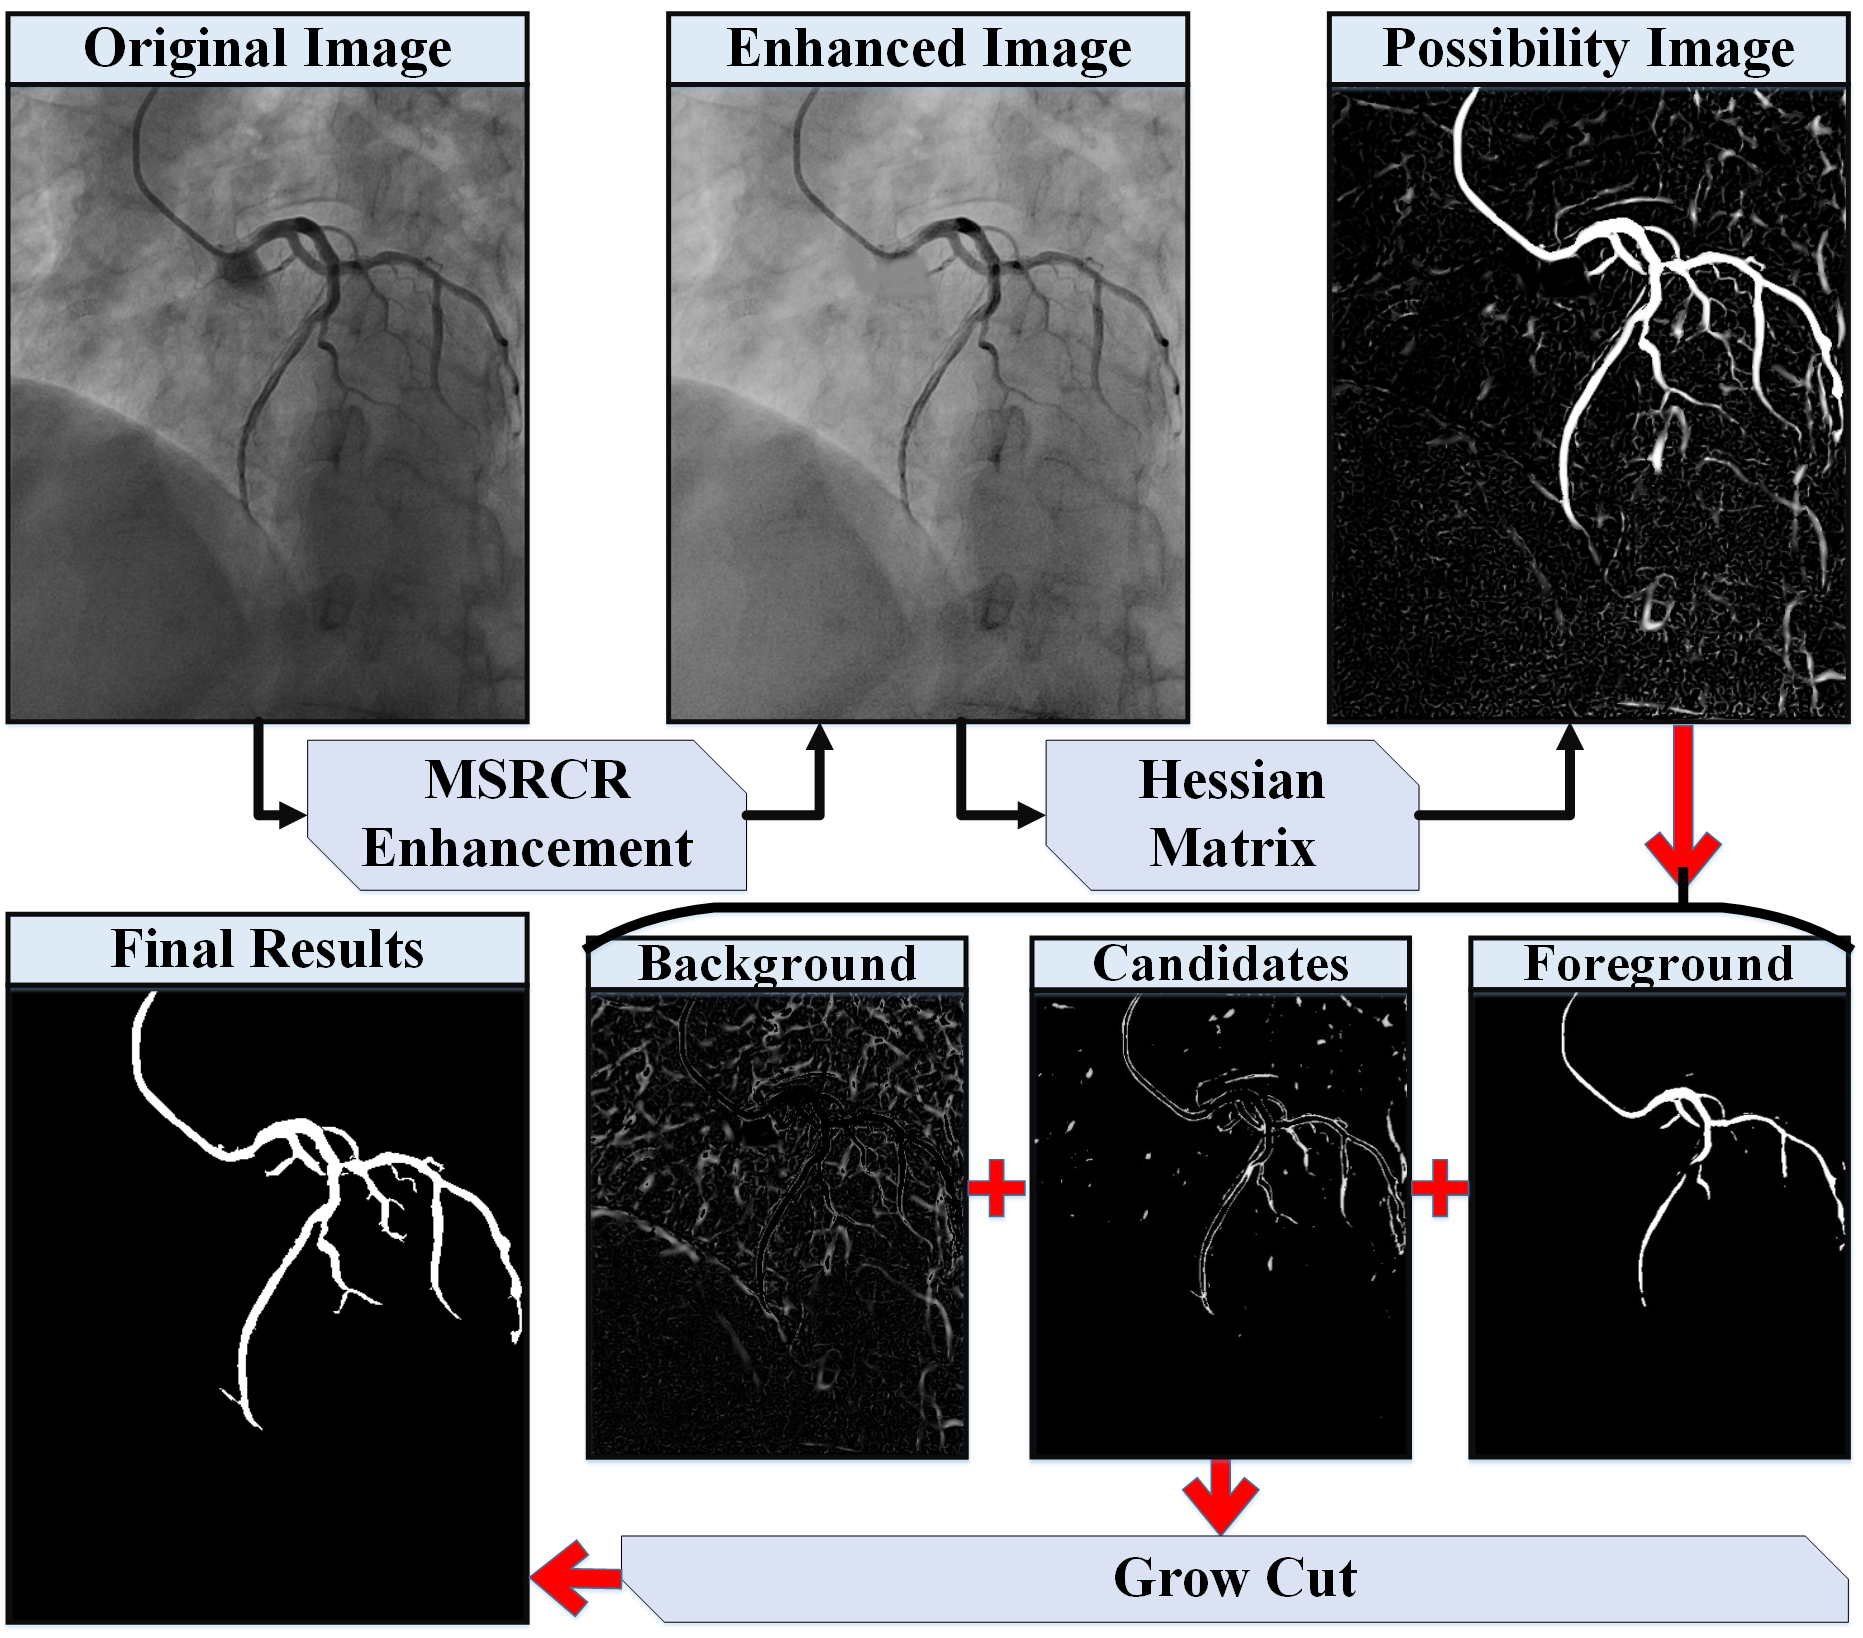
\includegraphics[width=1.0\linewidth]{./images/basis-pipeline.png}
\caption{Work pipeline for vessel extraction.}
\label{fig:pip_extraction}
\end{figure}

\subsubsection{\textbf{Angiogram Enhancement}}
We first apply the enhancement of radiography based on Musicale Retinex with Color Restoration(MSRCR)~\cite{rahman1996multi}. Then, we use the gain/offset method to fix the negative values. After the pre-processing procedure, original images are enhanced with better contrast and lumen, providing better basis for vessel extraction.

\subsubsection{\textbf{Candidates from Hessian Matrix}}
\label{subsubsec:hessian}
We compute the probability of being one of the vessel candidates for each pixel on the image using Hessian Matrix~\cite{Frangi}. We convolve original images by four Gaussian filters with different scales and compute the weighted average of them.

Since the computation on every pixel is independent, the vessel extraction algorithm is very suitable to be parallelized with mapping each pixel to a CUDA thread for parallelization. The sketch up for processing on GPU is described in Fig.~\ref{fig:hessian_gpu}. For every angiogram among the imaging sequence and for every specified $\sigma$, our parallelized extraction method consists of the following steps. First, we build the Gaussian kernel mask depending on $\sigma$ on CPU side and transfer them into the GPU. Then, we convolve the entire image using this Gaussian kernel and each pixel point on the image corresponds to one CUDA kernel. After that, we extract the eigenvalues and eigenvectors and compute the coefficients for each point's Hessian matrix. This is also done per kernel on GPU. Finally, we use a double swap buffer on GPU to compute the possibility of being part of vessel structures for each pixel(refer to Eq.~15 of~\cite{Frangi} for details). In all the procedures, except initialization, datas are processed on GPU side and stored for further processing.

\begin{figure}[!t]
\centering
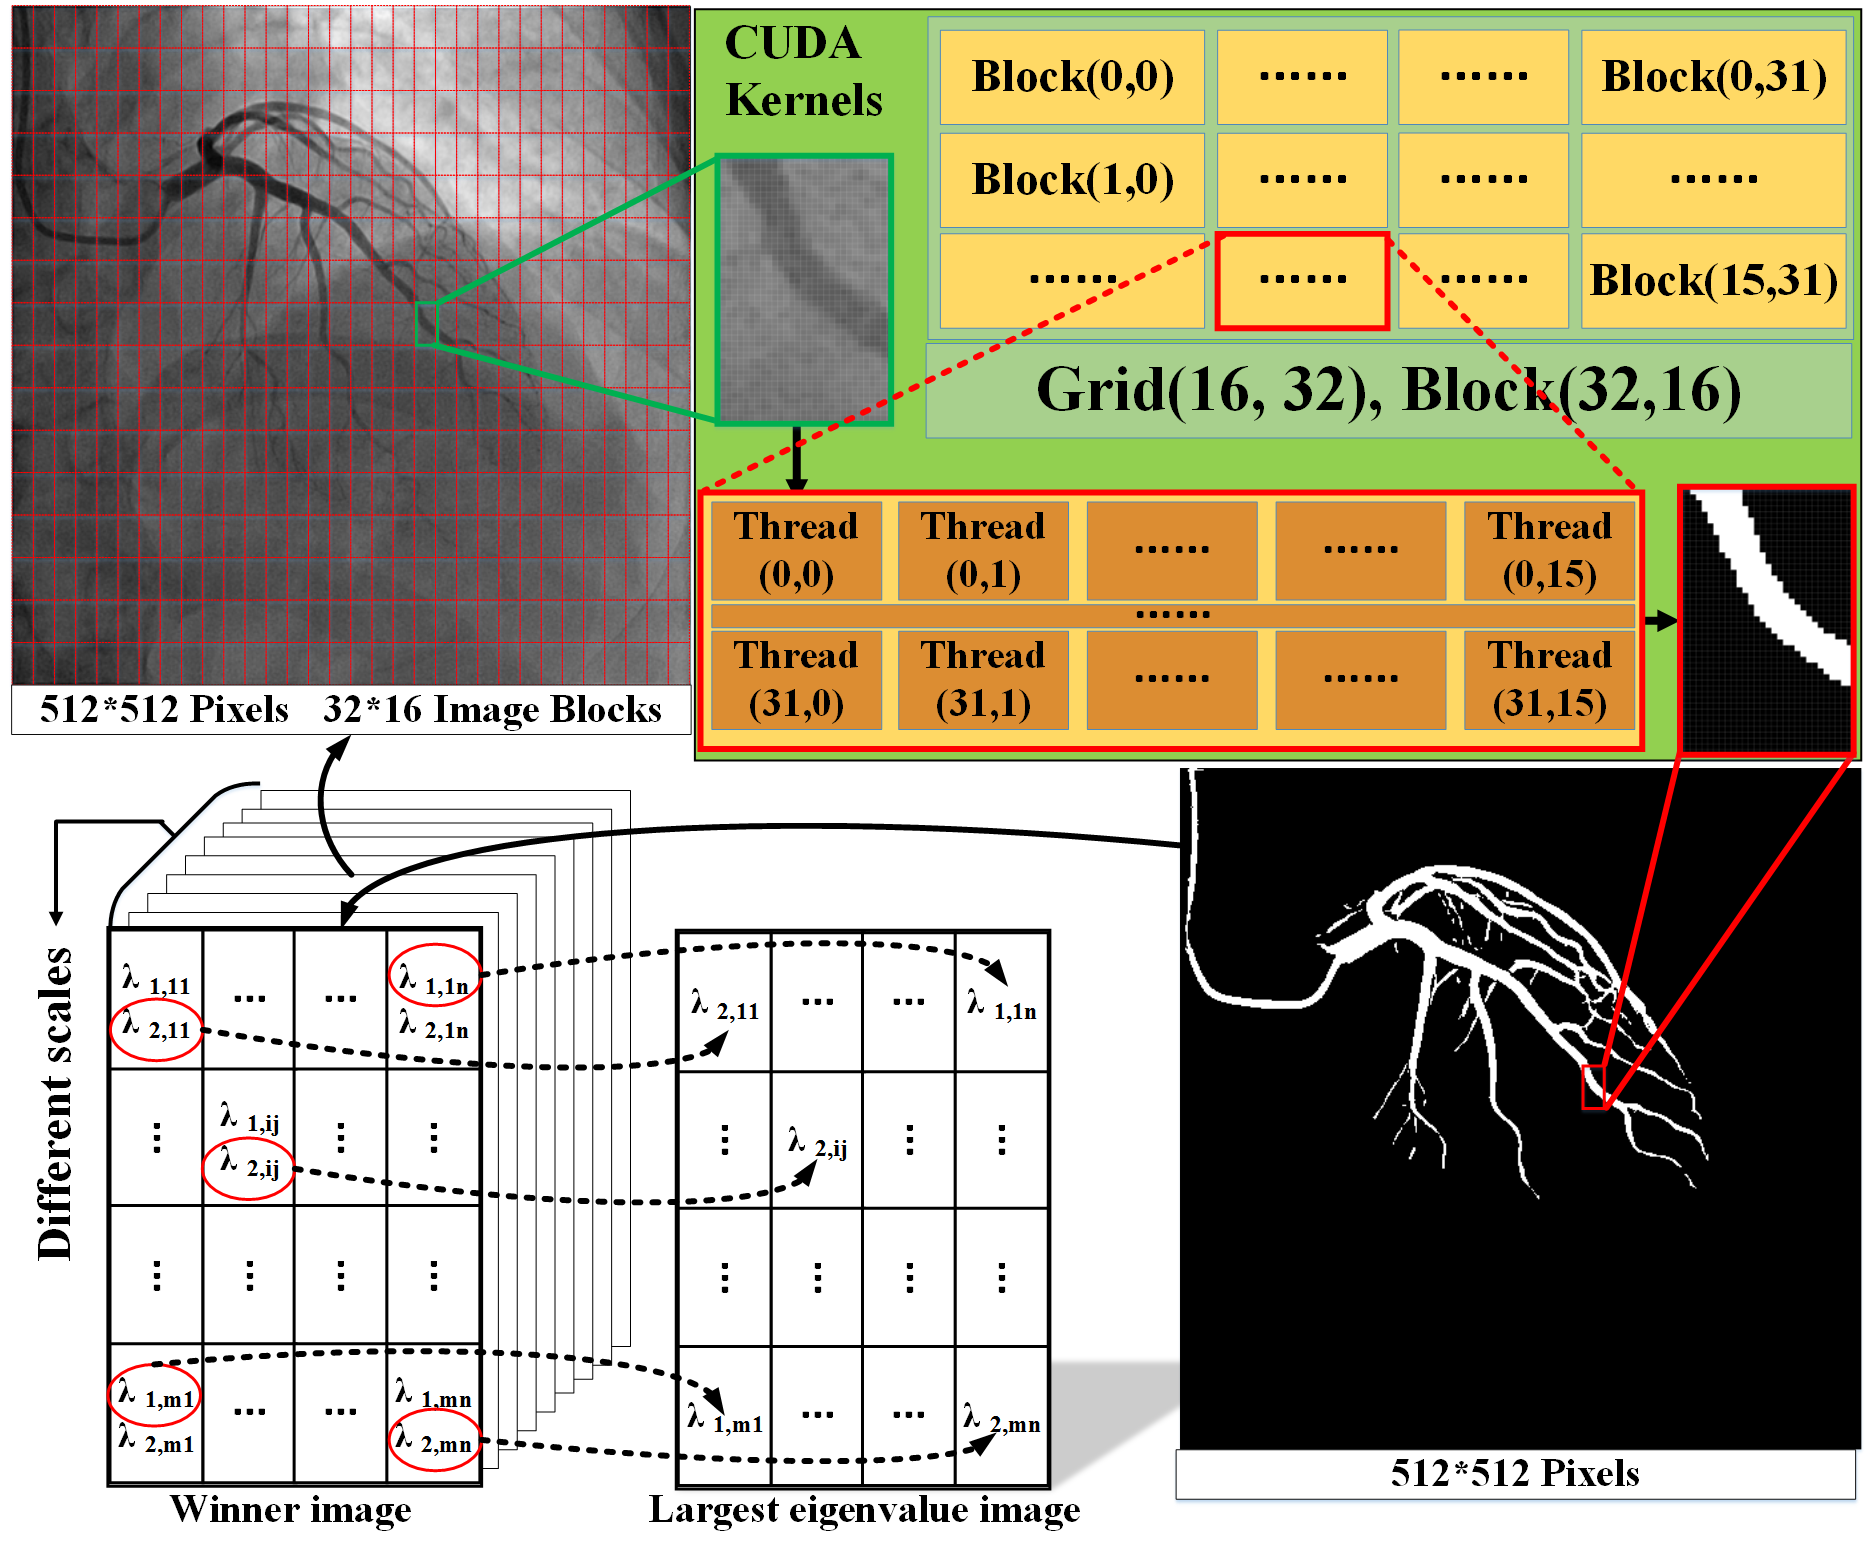
\includegraphics[width=1.0\linewidth]{./images/hessian_gpu.png}
\caption{Vessel extraction for single image on GPU.}
\label{fig:hessian_gpu}
\end{figure}

\subsubsection{\textbf{Precise Results using Grow Cut}}
\label{subsubsec:growcut}
Our precise segmentation for vessels mainly relies on the Grow Cut~\cite{vezhnevets2005growcut} method which is an alternative to Graph Cuts with much better performance. This method can be thought of being with a biological metaphor that each image pixel is formulated as a cell of certain type. These cells can be \textit{foreground}, \textit{background}, \textit{undefined} or others. As the algorithm proceeds, these cells compete to dominate the image domain. The ability of the cells to spread is related to the image pixel intensity.

Based on the probability image acquired from GPU-accelerated Hessian, we divide the candidates on the image into three categories: \textit{background}, \textit{foreground(vessel)} and \textit{undefined} pixels. For all pixels $p$ in the image, the processing stage mainly consist of two steps: firstly, current state and weighted strength from last iteration will be saved. Then, for all neighbours $q$ of pixel $p$, we will compute the new strength through multiplying $attack\_force$ by $strength$ and replace the old $strength$ if it is smaller than the new one. After that, all pixels in the image will be assigned with a label by $0$ and $1$, which means \textit{background} and \textit{foreground}. At last, We collect the \textit{foreground} pixels as vessel segments and calculate counts of each segment. Finally, segments whose point count is smaller than a given value are omitted and we achieve well clear vessel images which has been shown as \textit{Final Results} in Fig~\ref{fig:pip_extraction}.


\subsection{Skeleton Extraction}
\label{subsec:skeleton-extraction}
We use the Fast Marching method with second derivatives and cross neighbors to track the centerline of extracted vessels. This method is based on ~\cite{IMM2001-0841} and \cite{hassouna2007multistencils}. The pipeline is described in Fig.~\ref{fig:skel_extraction}. We will calculate the accurate skeleton of objects represented by binary images using the Fast Marching distance transform. Firstly, we compute the distance map for the whole binary image. Then, we will trace the shortest path from start point to source point using Runge Kutta method in the distance map. At last, we will organize and split traced points into line segments. With the help of both second derivatives and cross neighbours, we achieve segmented skeletons more accurate. Meanwhile, we extracted diameters for each skeleton point during the distance transform.

\begin{figure}[!t]
\centering
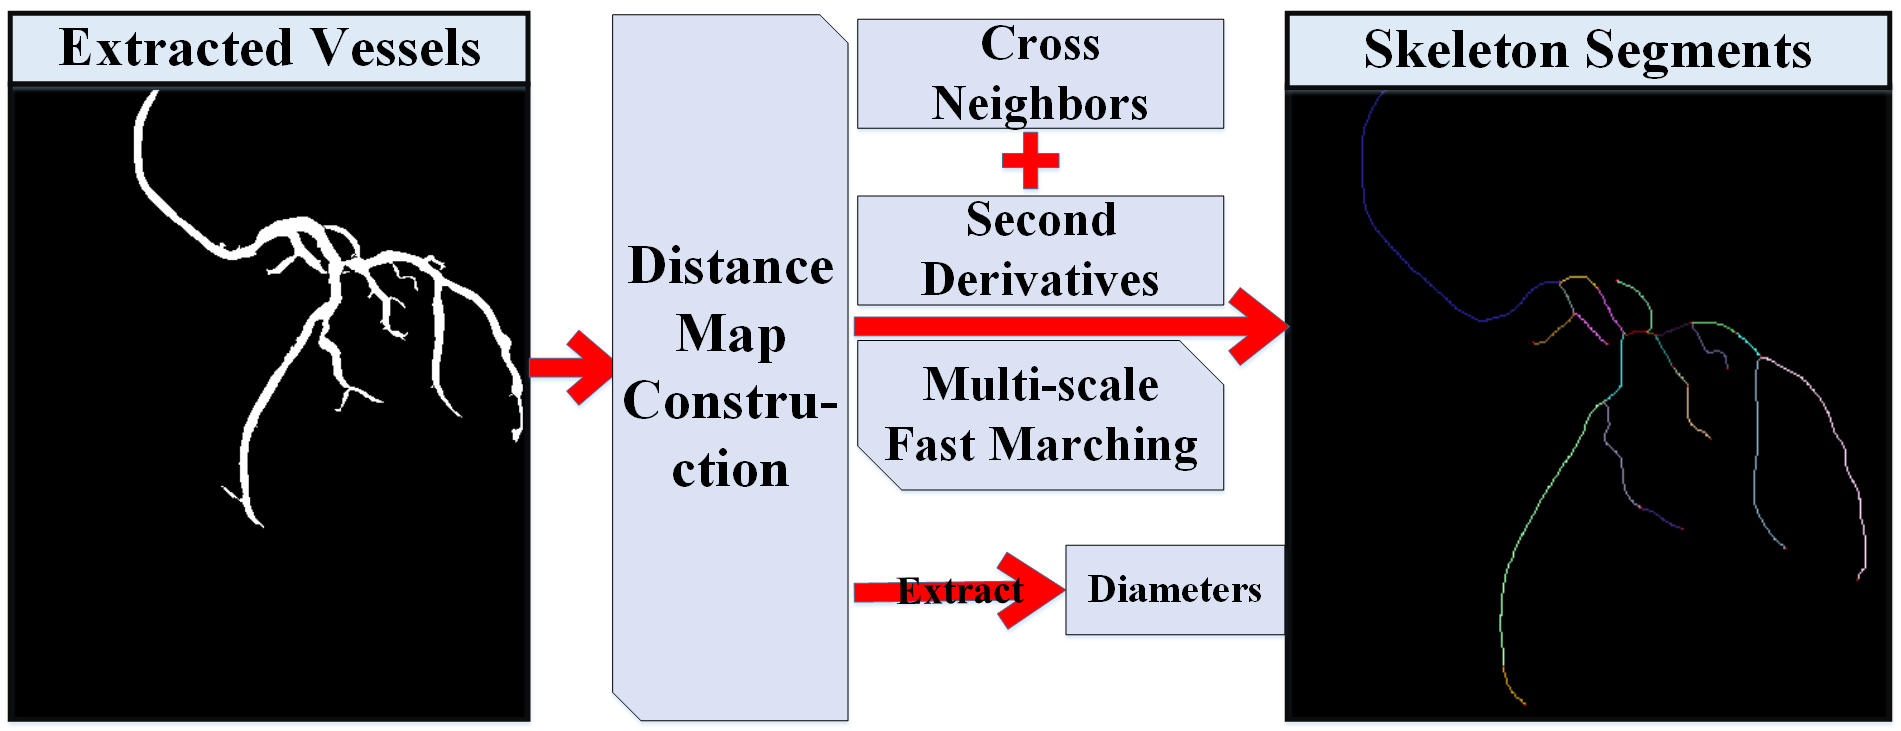
\includegraphics[width=1.0\linewidth]{./images/basis2-pipeline.png}
\caption{Work pipeline for skeleton extraction. Multistencils Fast Marching is used with cross neighbours and second derivatives to improve accuracy.}
\label{fig:skel_extraction}
\end{figure}

%%%%%%%%%%%%%%%%%%%%%%%%%%%%%%%%%%%%%%%%%%%%
\section{Vessel Organization}
\label{sec:vessel-organization}
Extracted vessel skeletons are messy segments composed of many pixels which are not structured. It is too difficult to label skeletons based on such type of data. Therefore, we divide the labeling problem into two sub-problems, which we call Vessel Organization(Section~\ref{sec:vessel-organization}) problem and Tree Structure Labeling(Section~\ref{sec:tree-labeling}) problem. In the first step, we organize the messy extracted skeleton points and segments, transforming them into well organized unique tree structures. The pipeline for organizing extracted skeletons is described in Fig.~\ref{fig:skel_organization} consisting of two steps.

\begin{figure}[!t]
\centering
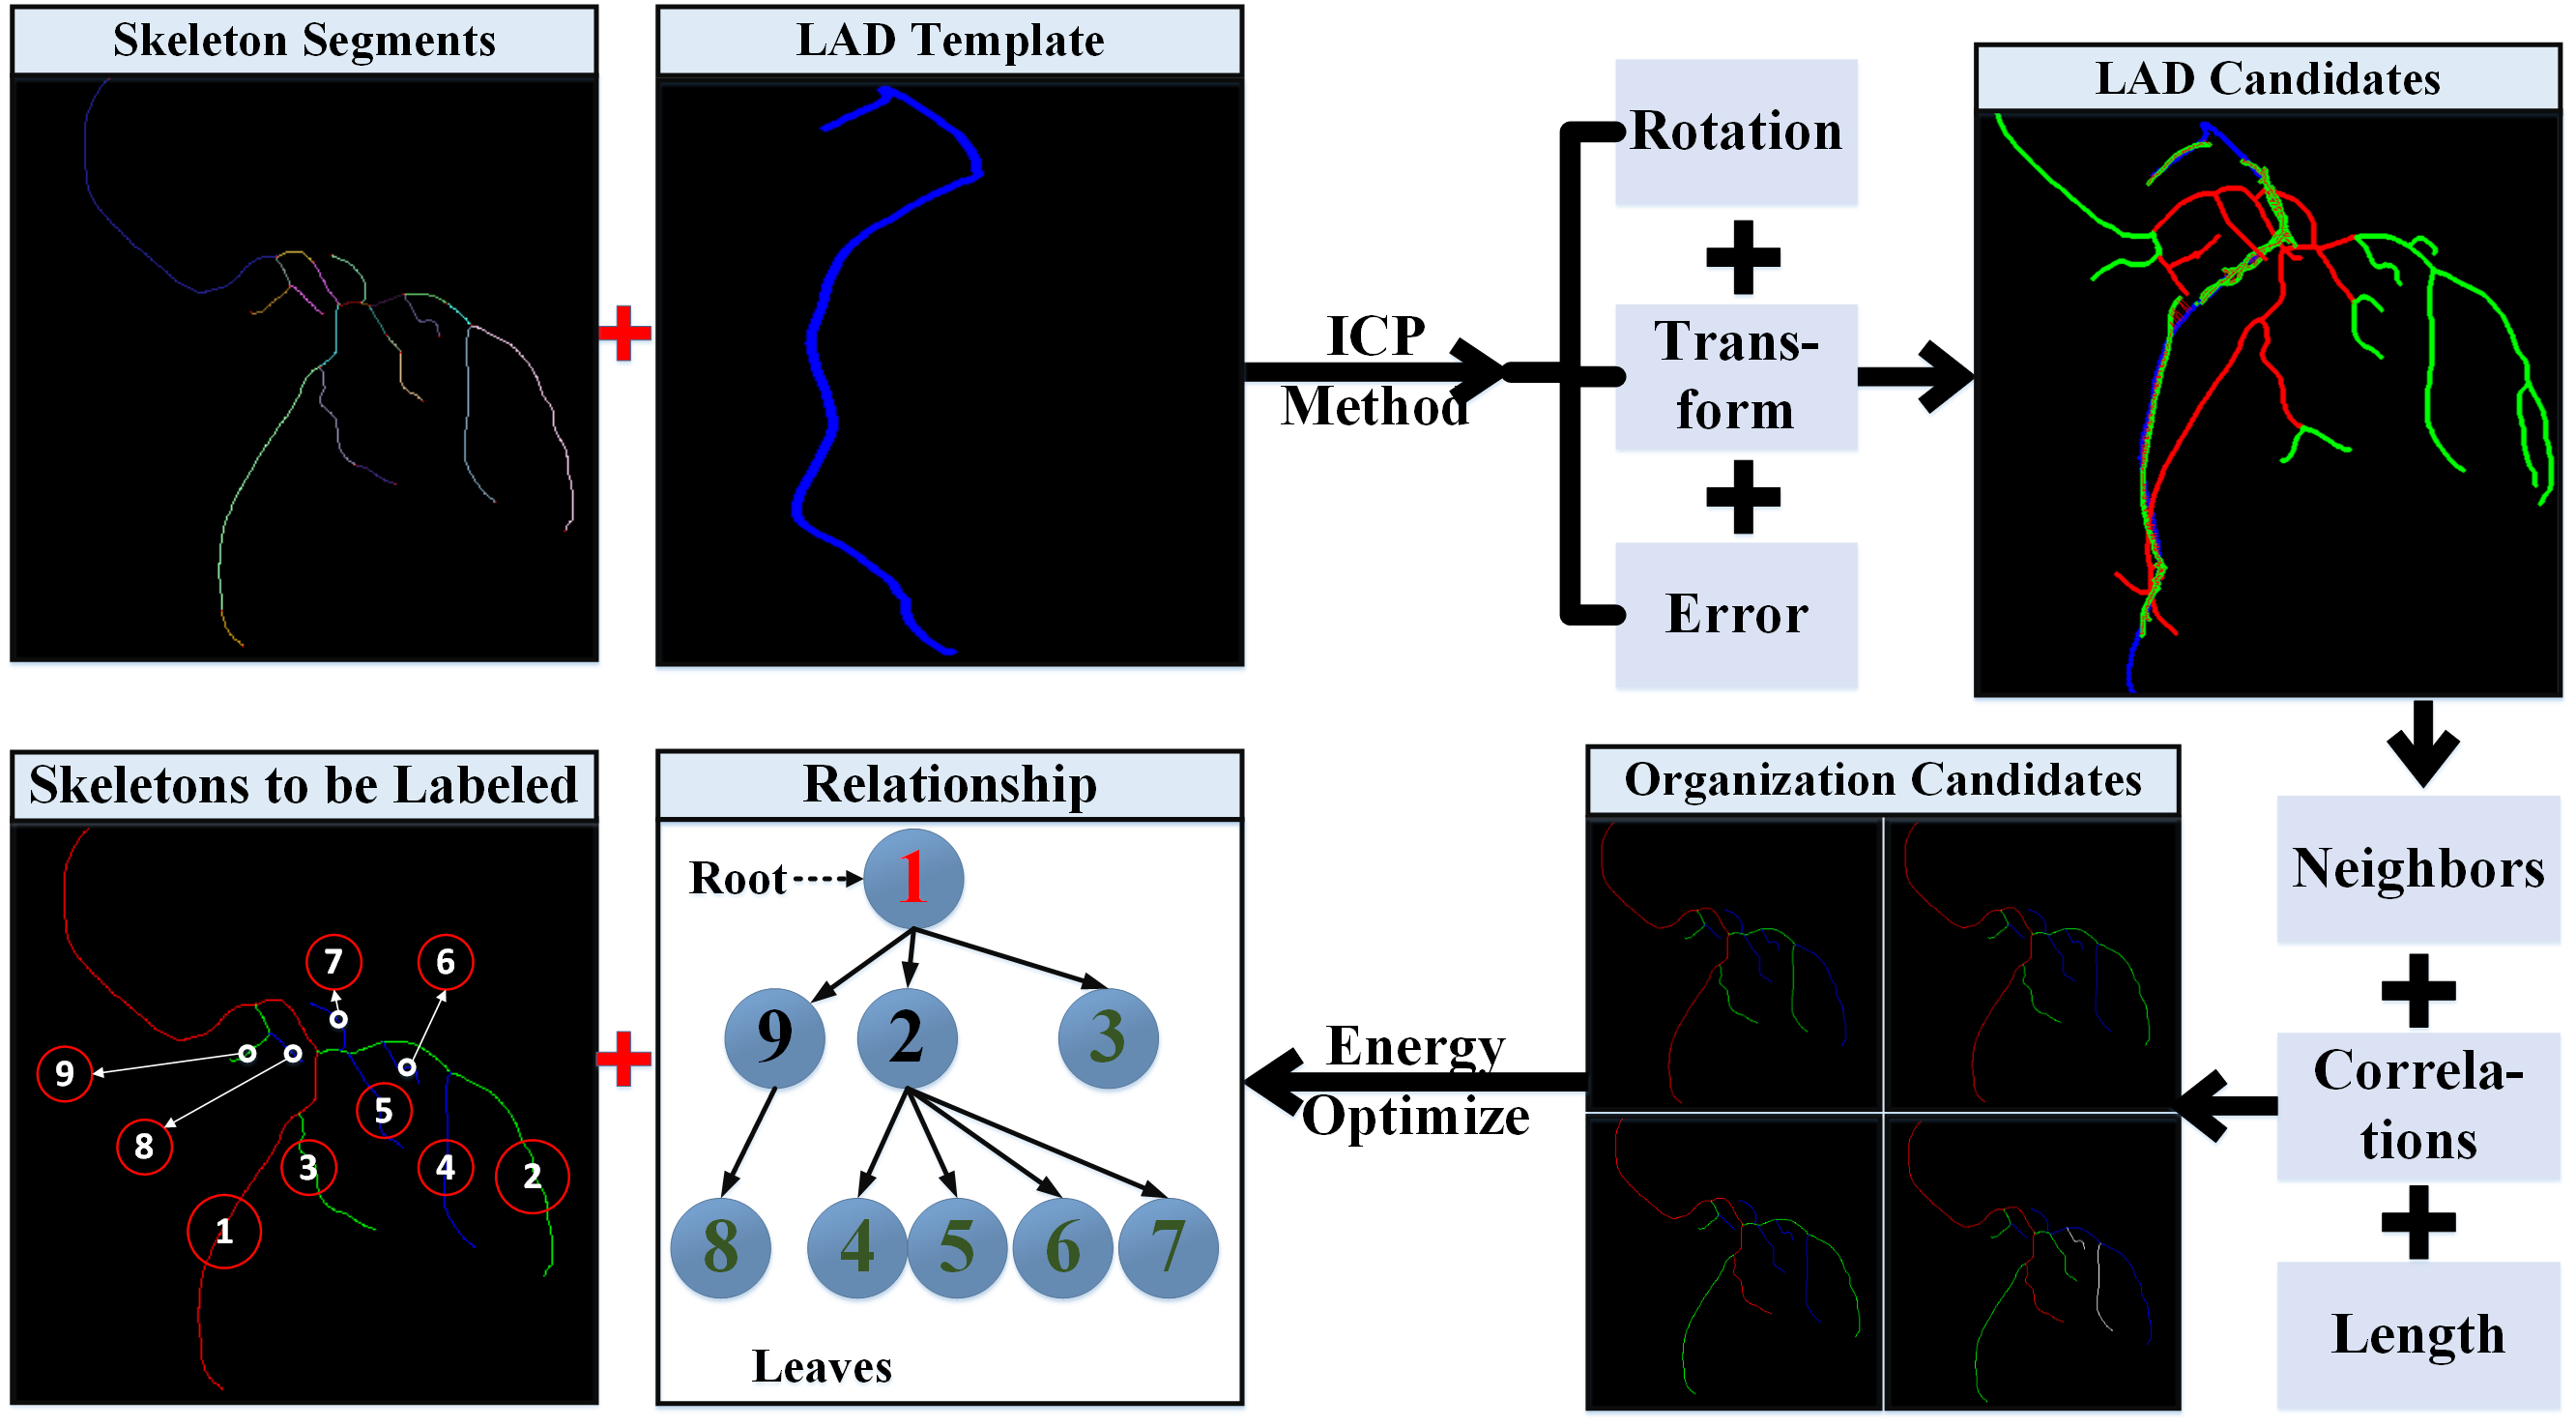
\includegraphics[width=1.0\linewidth]{./images/skel-orga-pipeline.png}
\caption{Work pipeline for skeleton organization. (a): Skeleton segments. (b): LAD template. (c): Candidates using LAD. (d): Different organized candidates. (e) and (f): Processed skeletons and relationship.}
\label{fig:skel_organization}
\end{figure}

\subsection{Landmark Building}
Coronary arteries are precisely tree structures with tree root, branches and leaves. It is very important to figure root and primary branches to build the right tree structure. Because of the particularity of vascular angiography, we mainly lay our attention on extraction and analysis of three landmarks including the \textit{Catheter}, the \textit{LAD} branch and the \textit{LCX} branch by the application of our ICP based method. The ground truth landmarks at a given angle are shown in Fig.~\ref{fig:step1_result}.

\subsubsection{\textbf{Catheter Building}}
In our application, we make sure the angiograms are taken at the very beginning of the intervention, when the catheter is inside the coronary artery and no contrast media is injected. Therefore, we can use our vessel extraction method to process the beginning several images in the sequence for catheter which will be ground truth in the following images. We use the \textit{transmission}, \textit{rotation} and \textit{error} parameters from ICP method as the evaluation distance for catheter comparison. The extracted catheter is shown in Fig.~\ref{fig:catheter_building}.

\begin{figure}[!t]
\centering
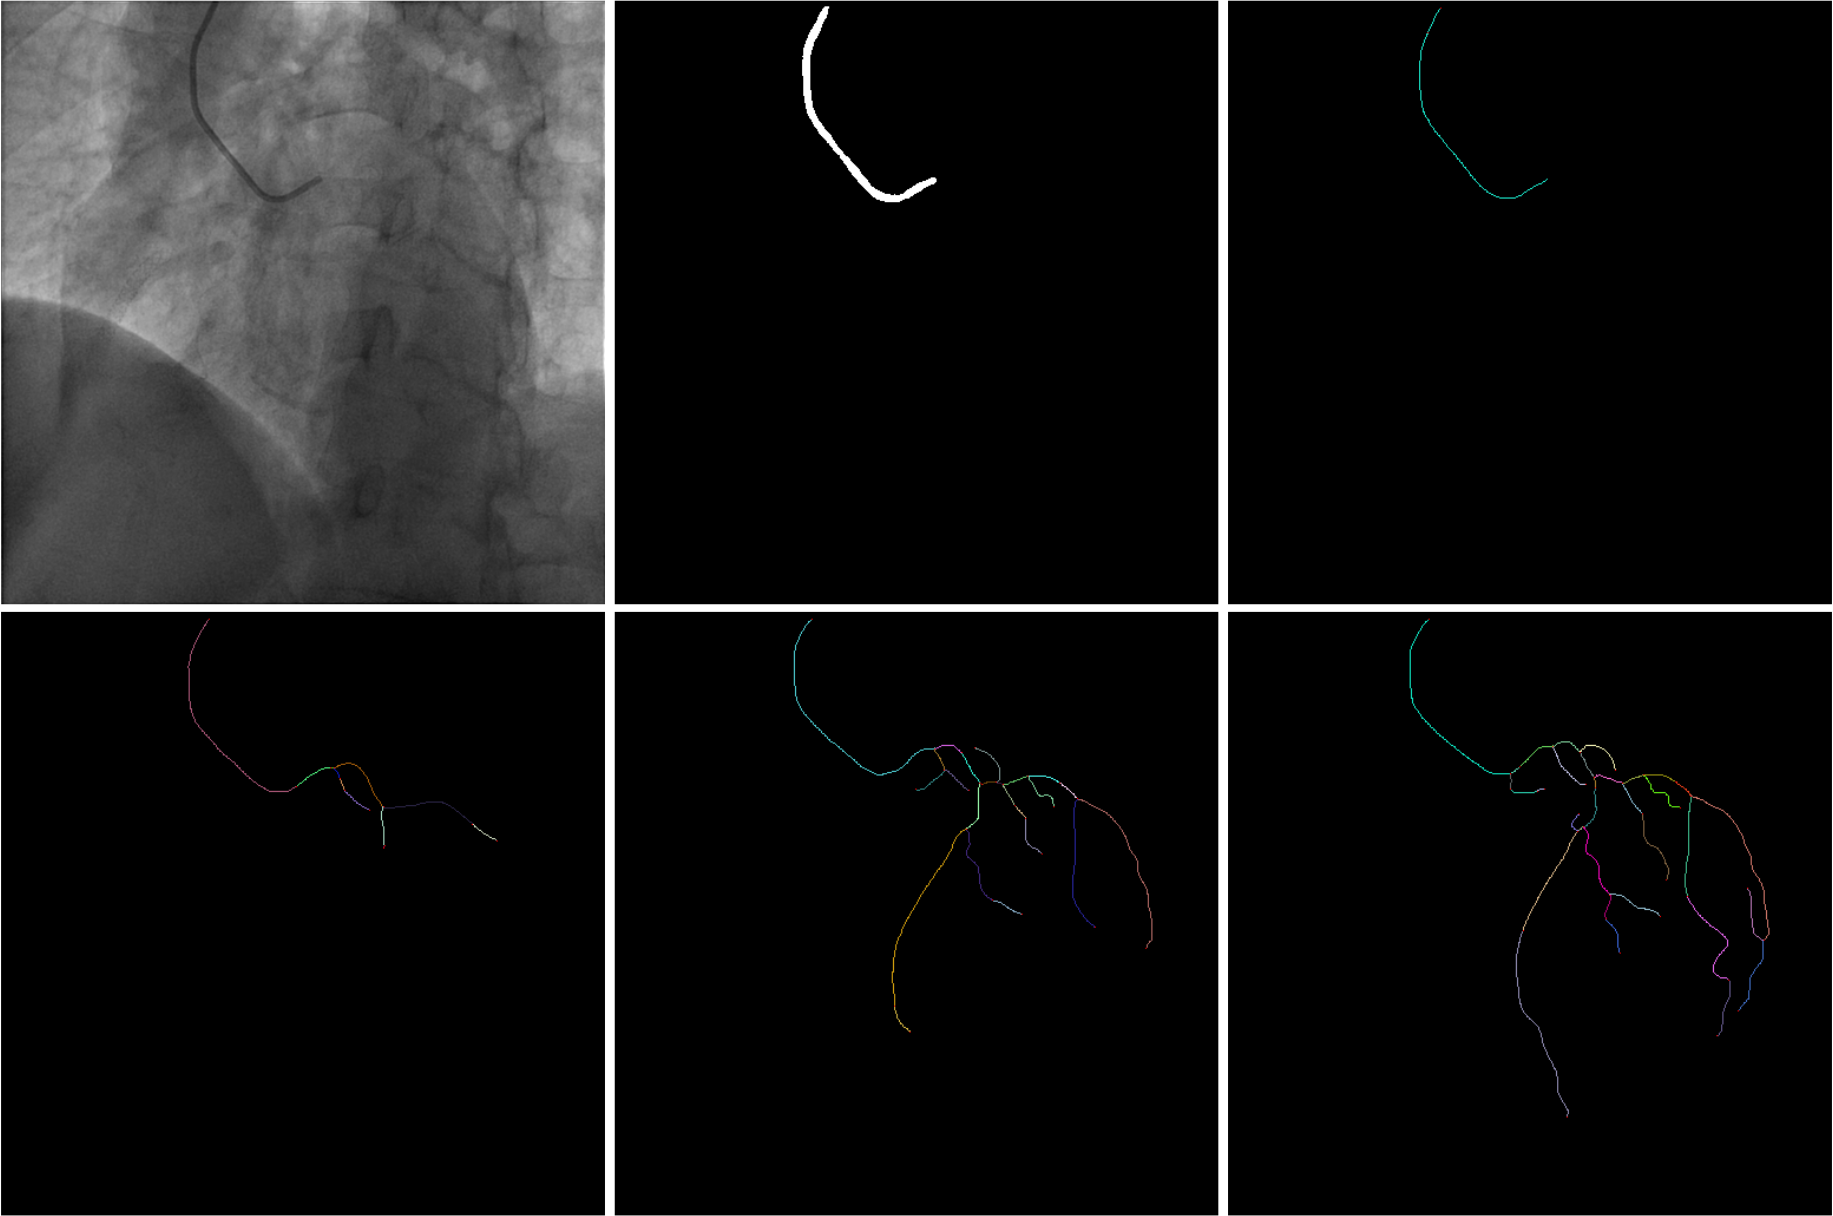
\includegraphics[width=1.0\linewidth]{./images/catheter_building.png}
\caption{Extracted catheters from the sequence. The top row: catheter from the beginning images of the sequence. The bottom row: traced catheters and other skeleton segments.}
\label{fig:catheter_building}
\end{figure}

\subsubsection{\textbf{LAD and LCX Building}}
LAD and LCX branches are also as important as the catheter. Since we have a known 3D ground truth, we can easily achieve the 2D projected geometrical and structural information of LAD and LCX which we call \textit{Template}. We take the template $t$ as ground truth and compute the similarity for each segment $s$ by $D_t(s)$ which is composed of ICP-returned parameters in the extracted image. The $D_t(s)$ is described as:

\begin{equation}
\label{eq:dp_fp}
\begin{split}
&D_t(s) = [(|L(s)/L(t)-1|+1)*(T(s)+Err(s)\\
&*THRE\_ICP)*(1+R(s)/180)]/Count(s),
\end{split}
\end{equation}

in which $L(s)$ stands for the length of segment $s$, $T(s)$, $Err(s)$ and $R(s)$ are parameters calculated for $s$ from ICP, $THRE\_ICP$ is a constant and $Count(s)$ stands for points count of segment $s$.

Once we calculate the $D_t(s)$ for each segment, we obtain corresponding segments for the template shown in Fig.~\ref{fig:skel_organization}(c). Meanwhile, since we build catheter from the messy segments, we have the straight issue for building LAD branch since catheter is directly intervened into the LAD branch. We start from the intersection segment and search for the neighbours for each working node until it is a distal node. As there are multiple distal nodes during searching, there are several options LAD may be. After LAD has been determined, the same procedure advances the same for LCX branch. Suppose there are $m$ choices for LAD and $n$ choices for LCX, there are totally $m \times n$ options for the whole combinations. We transform the messy data into vessel trees according to selected LAD and LCX(See Section~\ref{subsec:vessel-tree-building}), and iterate all the combinations, calculating the globally optimized energy(See Section~\ref{subsec:labeling-using-bp}) for each combination. At last, we select combination with minimal energy as the final structure. The whole algorithm is described in Algorithm~\ref{alg:icp_matching}.

\begin{algorithm}
  \caption{ICP Based Skeleton Segments Organization}
  \label{alg:icp_matching}
  \renewcommand{\algorithmicrequire}{\textbf{Input:}}
  \renewcommand{\algorithmicensure}{\textbf{Output:}}
  \begin{algorithmic}
  \Require ~~\\
    $Cath$, extracted catheter segments.\\
    $LADGr$, ground truth for LAD branch.\\
    $LCXGr$, ground truth for LCX branch.\\
    $LNodes$, to be labeled segments.
  \Ensure ~~\\
    segment combination with minimal energy.

  \Function {processOneImage}{()}
  \State $cathCandi \gets$ \Call{icpLookup}{$Cath$,$LNodes$}
  \State $iCath \gets$ $cathCandi$
  \State $LADCandi \gets$ \Call{icpLookup}{$LADGr$,$LNodes$}
  \State $vProcessed \gets$ insert $iCatheter$
  \State $LADs\gets$ \Call{collectPaths}{$LADCandi$,$Coeff$}

  \For{$m = 0 \to Count(LADs)$}
    \State $LCXCandi \gets$ \Call{icpLookup}{$LCXGr$, $LNodes$}
    \State $vProcessed \gets$ insert $LADs(m)$
    \State $LCXs \gets$ \Call{collectPaths}{$LCXCandi$,$Coeff$}
    \For{$n = 0 \to Count(LCXs)$}
        \State $vMerged \gets$ \Call{Merge}{$LADs(m),LCXs(n)$}
        \State $Energy \gets$ $vesselTreeBP(vMerged)$
    \EndFor
  \EndFor
  \State $minE,mMin,nMin \gets$ $min(Energy)$
  \State $finalMerged \gets$ \Call{Merge}{$LADs(mMin),LCXs(nMin)$}
  \EndFunction

  \Function {icpLookup}{$GNodes$, $LNodes$}
    \For{$i = 0 \to Count(LNodes)$}
       \State $Error \gets$ \Call{icp2D}{$GNodes$,$LNodes(i)$}
       \If{$Error<THRE$}
        \State $vCandi \gets$ $LNodes(i)$
       \EndIf
    \EndFor
    \State \Return $vCandi$
  \EndFunction

  \Function {collectPaths}{$LNodes$,$Coeff$}
  \State $Neis \gets$ \Call{getNeighbors}{$LNodes(k)$}
  \State $vRet \gets$ $empty$
    \For{$i = 0 \to Count(Neis)$}
        \If{!$IsProcc(Neis(i))$ and $IsCandi($Neis(i))}
            \If{$Corre(Neis(i))>THRE$}
                \If{$IsDistal(Neis(i))$}
                    \State $vRet \gets$ $Neis(i)$
                \Else
                     \State $vRet \gets$ $Neis(i)$
                     \State \Call{collectPaths}{$LNodes(Neis(i))$}
                \EndIf
            \EndIf
        \EndIf
    \EndFor
    \If{$Count(Neis)==0$ and $IsDistal(Neis(i))$}
        \State \Return $vRet$
    \EndIf
  \EndFunction
  \end{algorithmic}
\end{algorithm}

\subsection{Segments Organization}
As soon as LAD and LCX segment are determined, we can organize the rest segments clearly. The structured LAD, LCX and other segments are shown in Fig.~\ref{fig:segments_orga_result}. The rest segments are organized in an easy way based on the correlation $Corr(p,q)$ between neighboring segments $p$ and $q$ and is define as:

\begin{equation}
Corr(p,q) = \arctan \Bigg(\frac{|S(p)-S(q)|}{(1+S(p)*S(q))}\Bigg),
\end{equation}
where $S(p)$ denotes average slope value for skeleton $p$ and is defined as:

\begin{equation}
S(p) = \frac{N*\sum\limits_{i=1}^{N}{(X_p(i)*Y_p(i))}-(\sum\limits_{i=1}^{N}{X_p(i)})*(\sum\limits_{i=1}^{N}{Y_p(i)})}
{N*\sum\limits_{i=1}^{N}{(X_p(i)*X_p(i))}-(\sum\limits_{i=1}^{N}{X_p(i)})*(\sum\limits_{i=1}^{N}{X_p(i)})},
\end{equation}
where for each skeleton segment $p$, $N$ denotes the point count, $X_p$ and $Y_p$ represent the X-coordinate and Y-coordinate. In our application, we also define a minimal sample point count as $NORM\_AVGCount$. Once $N$ is smaller than $NORM\_AVGCount$, $Corr(p,q)$ is slightly enhanced as $Corr(p,q) = Corr(p,q)*(0.5+(1-N/NORM\_AVGCount))$ to give smaller segments better chances of merging into longer ones.

We start from a random skeleton segment and group the neighbors of current working segment with high correlation recursively. After each group is processed, we continue searching from the other uncovered segment until all segments have been covered. At last, segments belong to the same group will be merged into a new segment, the points belonging to each old segment will be queued and sorted by its location and the starting point and end point for this new segment will be refreshed. After the organization, we obtain a totally new structure with more reasonable, continuous segments and less small skeleton fragments.

\begin{figure}[!t]
\centering
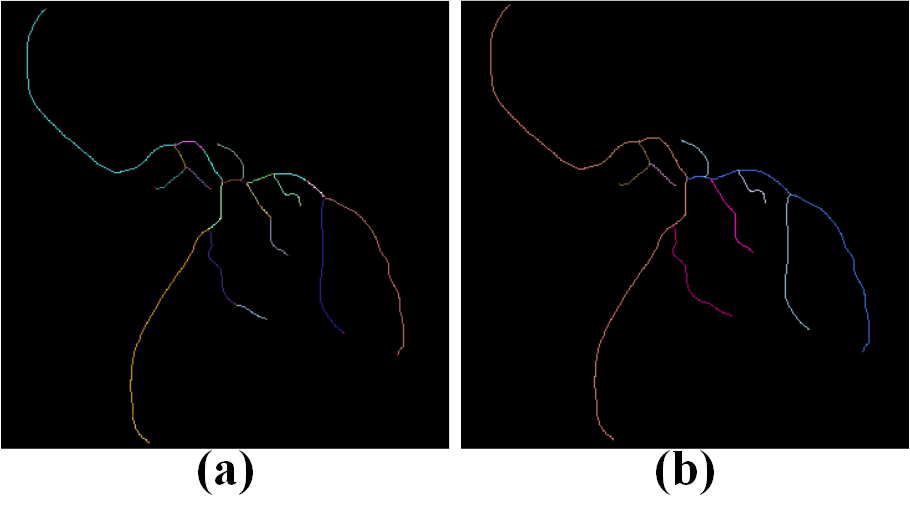
\includegraphics[width=1.0\linewidth]{./images/segments_orga_result.png}
\caption{Results for vessel organization. (a): Messy vessel segments. (b): Organized vessel segments.}
\label{fig:segments_orga_result}
\end{figure}

%%%%%%%%%%%%%%%%%%%%%%%%%%%%%%%%%%%%%%%%%%%%
\section{Tree Structure Labeling}
\label{sec:tree-labeling}
After the messy segments have been transformed into well organized structures, we further process the structure into vessel trees to which our following energy optimization method is applied. Our method of tree structure labeling can be described in Fig.~\ref{fig:tree-labeling} mainly consisting of three steps: vessel tree building(Section.~\ref{subsec:vessel-tree-building}), 3D ground truth projection and labeling the tree structure(Section.~\ref{subsec:labeling-using-bp}).

\begin{figure}[!t]
\centering
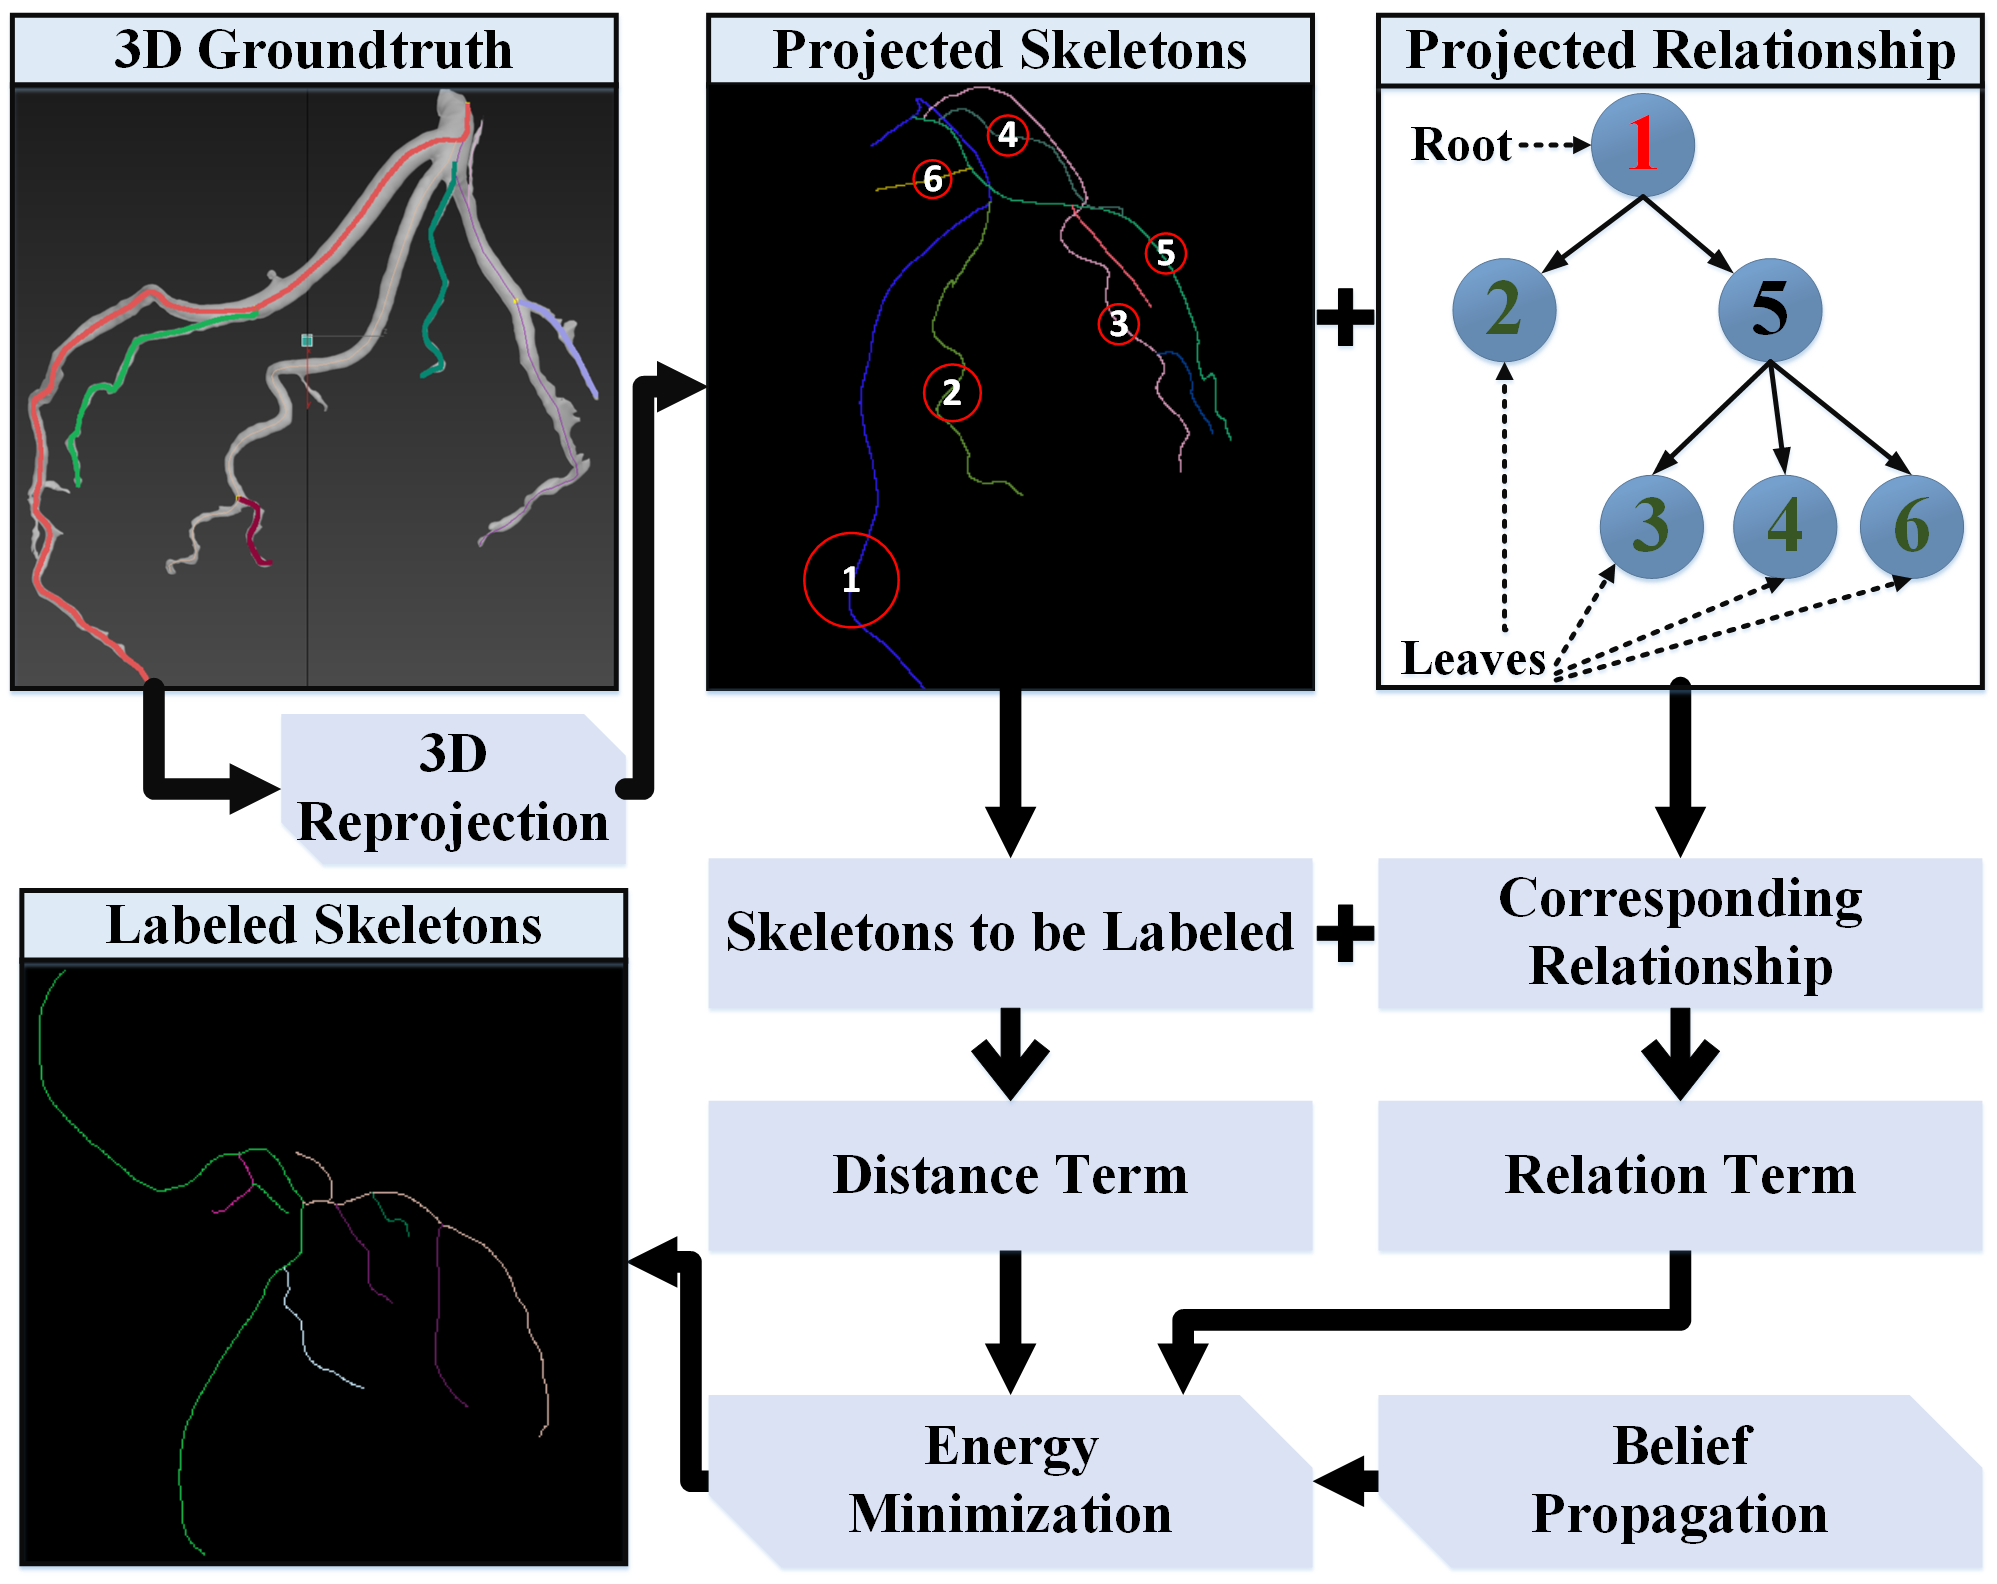
\includegraphics[width=1.0\linewidth]{./images/labeling-pipeline.png}
\caption{Work pipeline for vessel tree labeling.}
\label{fig:tree-labeling}
\end{figure}

\subsection{Vessel Tree Building}
\label{subsec:vessel-tree-building}
We build the vessel tree from each organized vessel structures. Each tree node corresponds to a vessel segment in which LAD and LCX are corresponding to root node and one of the primary branch separately. During the building, we compute the depth and neighborhood and parent-child relationship for each tree node based on depth-first iteration. The building procedure is described in Algorithm.~\ref{alg:vessel_tree_building}.

First, we collect the merged skeletons and analyze key points including bifurcations and distal nodes as input. Then, we build parent-child relationship between segments based on two-tuples($i,ptK$) which specify that it is a bifurcation point $ptK$ on segment $i$. After that, we assign each node with a unique code which is composed of the inherent code from its parent and the unique code of itself. This code enables us to compute the minimal path between nodes efficiently. Finally, we will analyze if the node is a distal node with less than one bifurcation or a inner node with two bifurcations through looking up in the bifurcation table. After all these analysis, we will iterate all nodes depth-first and record both the depth and the root nodes.

\begin{algorithm}
  \caption{Vessel Tree Building}
  \label{alg:vessel_tree_building}
  \renewcommand{\algorithmicrequire}{\textbf{Input:}}
  \renewcommand{\algorithmicensure}{\textbf{Output:}}
  \begin{algorithmic}[]
  \Require ~~\\
    $szNodes$, size of merged segments.\\
    $mSegs$, merged segments.\\
    $mBifs$, merged bifurcations. \\
    $mCuts$, two-tuples($i,ptK$), specify bifurcation $ptK$ on $i-th$ segment
  \Ensure ~~\\
    built vessel tree.
  \State
  \Function {buildTree}{$mSegs$,$mBifs$,$mCuts$}
    \State $Rels \gets$ \Call{buildRelation}{$mSegs$,$mBifs$,$mCuts$}
    \For{$i = 0 \to Count(Rels)$}
      \State $sSRC \gets$ $mSegs(Rels(i)(0))$
      \State $sTAR \gets$ \Call{find}{$mBifs(Rels(i)(1))$}
      \State $sSRC.child \gets$ insert $sTAR$
      \State $sTAR.parent \gets$ $sSRC$
    \EndFor

    \For{$i = 0 \to Count(mSegs)$}
      \State $biST \gets$ \Call{IsBifur}{$mSegs(i)(0)$}
      \State $biEnd \gets$ \Call{IsBifur}{$mSegs(i)(1)$}
      \If{!$biST$ and !$biEnd$}
        \State $mSegs(i).type \gets$ $Distal$
      \Else
        \State $mSegs(i).type \gets$ $Inner$
      \EndIf
    \EndFor
    \State \Return $vCandi$
  \EndFunction
  \State
  \end{algorithmic}
\end{algorithm}

\subsection{Labeling using Belief Propagation}
\label{subsec:labeling-using-bp}
It is very proper to apply the energy based method to the tree-structured vessels with global optimization nature. Our labeling procedure is described in Algorithm.~\ref{alg:vessel_tree_labeling}.

\begin{algorithm}
  \caption{Vessel Tree Labeling}
  \label{alg:vessel_tree_labeling}
  \renewcommand{\algorithmicrequire}{\textbf{Input:}}
  \renewcommand{\algorithmicensure}{\textbf{Output:}}
  \begin{algorithmic}[]
  \Require ~~\\
    $szNodes$, size of merged segments.\\
    $mSegs$, merged segments.\\
  \Ensure ~~\\
    built vessel tree.
  \State
  \Function {vesselTreeBP}{$mSegs$,$mBifs$,$mCuts$}
   
  \EndFunction
  \State
  \end{algorithmic}
\end{algorithm}

In our application, the energy term is defined as:
\begin{equation}
E(f) = \sum_{p\in P} D_{p}(f_{p}) + \lambda \sum_{p,q \in N} V_{p,q}(f_{p}, f_{q}).
\end{equation}

where $p$ represents each node on the vessel tree, $N$ denotes all neighbors of $p$ and $q$ denotes one of the neighbors.

We define $D_{p}(f_{p})$ as the minimal normalized value the same as Equation.~\ref{eq:dp_fp}, which we call as a \textit{Distance Term}:
\begin{equation}
D_{p}(f_{p}) = norm(min(D_{t}(f_{p})))
\end{equation}

Meanwhile, We define the $V_{p,q}(f_{p}, f_{q})$ as the \textit{Relationship Term} to ensure the continuity between adjacent segments $p$ and $q$. This term is related to the path length between the node $p$ and its ground truth node $f_{p}$. We define $V_{p,q}(f_{p}, f_{q})$ as:
\begin{equation}
V_{p,q}(f_{p}, f_{q}) = (1+\frac{nRouteCount-1}{MAX\_DEPTH})*(D_{p}(f_{p}) + D_{q}(f_{q})),
\end{equation}
where $nRouteCount$ denotes the path length from corresponding ground truth node $f_{p}$ to node $f_{q}$, $MAX\_DEPTH$ denotes the maximum depth iterated from the tree. Since message propagation is processed between neighboring nodes, they have relationships including both parent-child and siblings. Therefore, larger $nRouteCount$ can easily penalize labels not well fit on ground truth.

Once we have the \textit{Distance Term} and the \textit{Relationship Term}, we find the minimum $E(f)$ using Belief Propagation(BP) algorithm, which is composed of two main steps, message propagation and energy minimization. In the message propagation step, we formulate the message propagated between nodes at the $t$ iteration as:
\begin{equation}
\begin{split}
&m_{p \to q}^{t}(f_{q}) = min(\alpha*D_p(f_{p}) + \beta*V_{p,q}(f_{p},f_{q}) + \\
&\gamma*\sum_{s \in N(p)\backslash q}{m_{s \to p}^{t-1}(f_{p})}),
\end{split}
\end{equation}
where $\alpha$, $\beta$ and $\gamma$ are constants controlling the weight of different components. $N(p)\backslash q$ represents all neighbors for segment $p$ except $q$.

We compute the message propagated to neighbor $q$ from each source node $p$. With a given $q$, we compute the minimum energy for each $p$ to make the message minimal. Since the domain of the definition of both $p$ and $q$ is the $k$ labels, the time complexity of computing message from $p$ to $q$ is $O(k^2)$. And if there are $n$ nodes, the whole propagation time should be $O(nk^2)$. And if there are
$T$ iterations before the energy converges, the time is finally $O(nTk^2)$.

After $T$ iterations we compute the belief vector as:
\begin{equation}
b_{q}(f_{q}) = D(f_{q}) + \sum_{p \in N(q)}{m_{p \to q}^{T}(f_{q})},
\end{equation}
In the end, we compute the minimum sum of all grouped vessel skeleton segments and obtain the optimal solution for the whole structured vessel tree.


%%%%%%%%%%%%%%%%%%%%%%%%%%%%%%%%%%%%%%%%%%%%
\section{Application}
Our proposed method can definitely label different segments with specialized semantics in medical imaging. Therefore, our method can be easily used to lots of analysis and diagnosis related to heart disease. We have taken three applications which can be described in Fig.~\ref{fig:application-pipline} to validate the the correctness and scalability of our method.

\begin{figure}[!t]
\centering
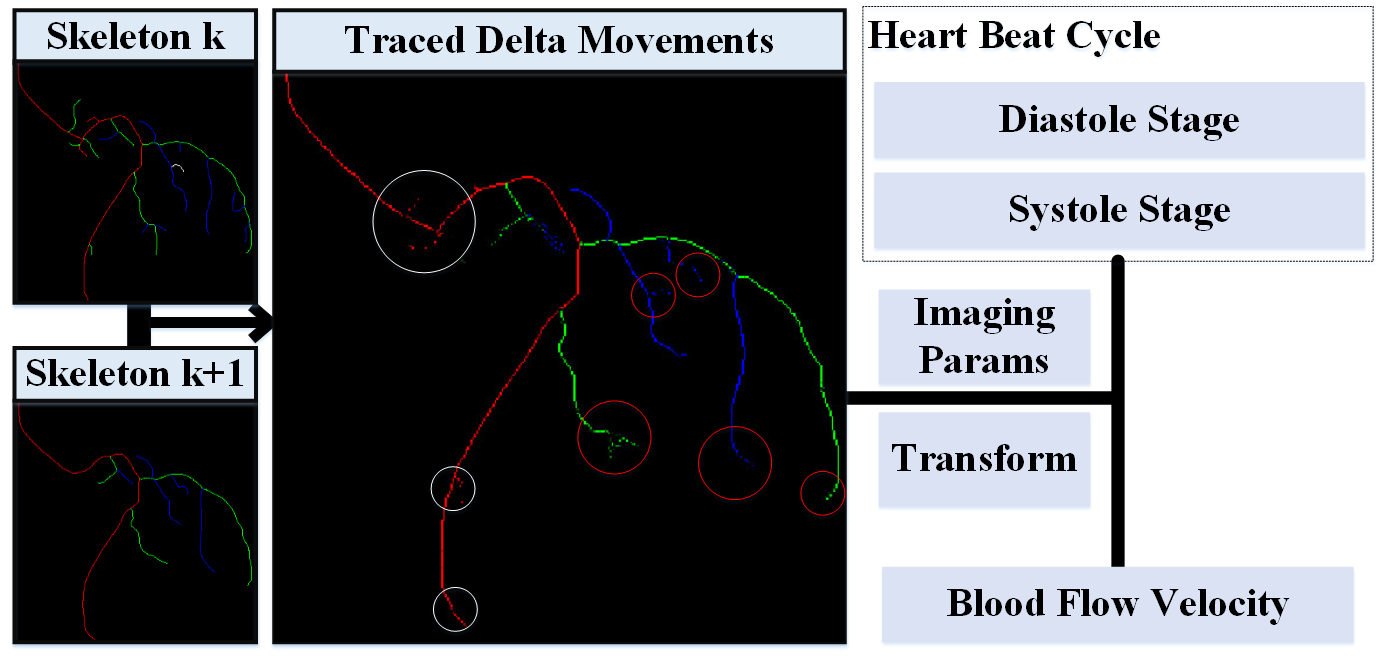
\includegraphics[width=1.0\linewidth]{./images/application-pipeline.png}
\caption{Work pipeline for vessel tree labeling.}
\label{fig:application-pipline}
\end{figure}

Once we obtain the correspondence between images and the ground truth or correspondence between images in the same sequence, we can calculate the corresponding delta movements on 2D images which later we can transform into 3D space to achieve real values with the inner parameters of the X-ray machine. It is perspective projection for X-ray machine from optical center to intensifier through humans in the middle which is described in Fig.~\ref{fig:application-sketchup}. The \textit{LAO, RAO, CRA} and \textit{CAUD} indicate the rotation of C-arm in 3D space. The distance of $D_{I2H}$ and $D_{O2H}$ are separately corresponding to distance from the intensifier to human and distance from optical center to human.

\begin{figure}[!t]
\centering
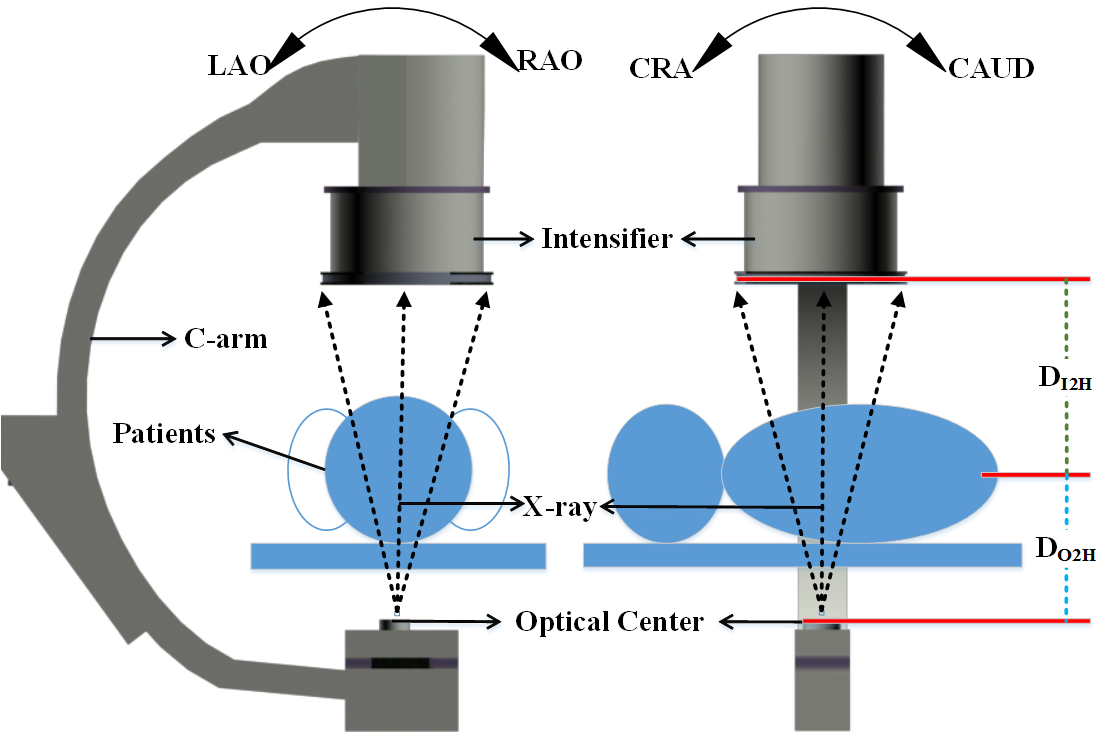
\includegraphics[width=1.0\linewidth]{./images/laorao.png}
\caption{Sketch up for X-ray inner parameters}
\label{fig:application-sketchup}
\end{figure}

\label{sec:application}
\subsection{Vessel Diameter Estimation and Analysis}
The diameter of vessels is an important sign for disease, especially for heart-related disease, such as vessel stenosis. On the other hand, diameters for each coronary artery owe a standard numerical value. Collecting and analyzing diameters from the X-ray images will be strong basis for doctors' diagnosis. In our application, we collect the diameters for all the extracted vessels and provide advice and assistance for diagnosis by calculating the distance map on binary images. We analyze the diameters and figure out nodes whose diameters are abnormal compared with their neighbors. We provide numerical analysis as well as graphical analysis shown in Fig.~\ref{fig:app_diameter_analysis} for better diagnosis.

\begin{figure}[!t]
\centering
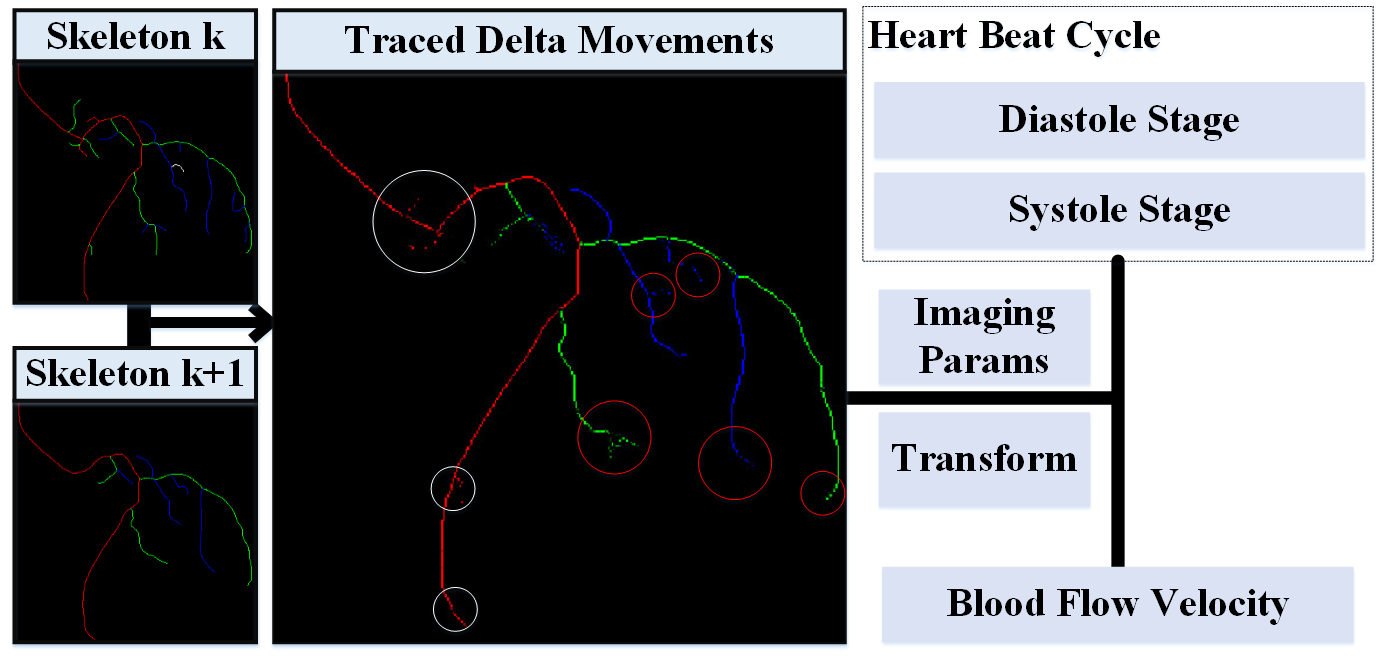
\includegraphics[width=1.0\linewidth]{./images/application-pipeline.png}
\caption{Numerical and graphical analysis for vessel diameters.}
\label{fig:app_diameter_analysis}
\end{figure}

\subsection{Flow Velocity Estimation and Analysis}
Flow velocity of coronary arteries is also an significant sign for any heart-related disease. Current methods collecting flow velocity statistics are mainly based on measurements from medical instruments. In fact, these kinds of methods require a catheter into the patients' coronary arteries, not only complicated and hard to be operated, but also sometimes not accurate either. The starting point of our this application is to select those who probably have stenosis with un-regular flow speed.

In our application, we label frame $t$ and frame $t+1$ in the same sequence based on our proposed method so that we can obtain the corresponding structure $S_{t}(p)$ and $S_{t+1}(q)$ in neighboring frames. Based on these corresponding structures, we achieve delta movements between frames which enables us to compute both the instantaneous movement speed for each segment and the average speed for whole structures. 

\subsection{Heart Beat Rate Estimation and Analysis}
Current methods using X-ray angiograms as input sources such as vessel extraction, 3D reconstruction will always require the cardiogram corresponding with the image sequences.This increases the requirements and decrease the applicability of these methods. In our application, we solve this problem using our labeling method. By analyzing the movement trend of each vessel tree node between the neighboring images in the same sequence, we can automatically extract the systole period and diastole period in the sequence. One full cardiac cycle has been shown in Fig.~\ref{fig:app_cardiac_cycle}. 

\begin{figure*}[!t]
\centering
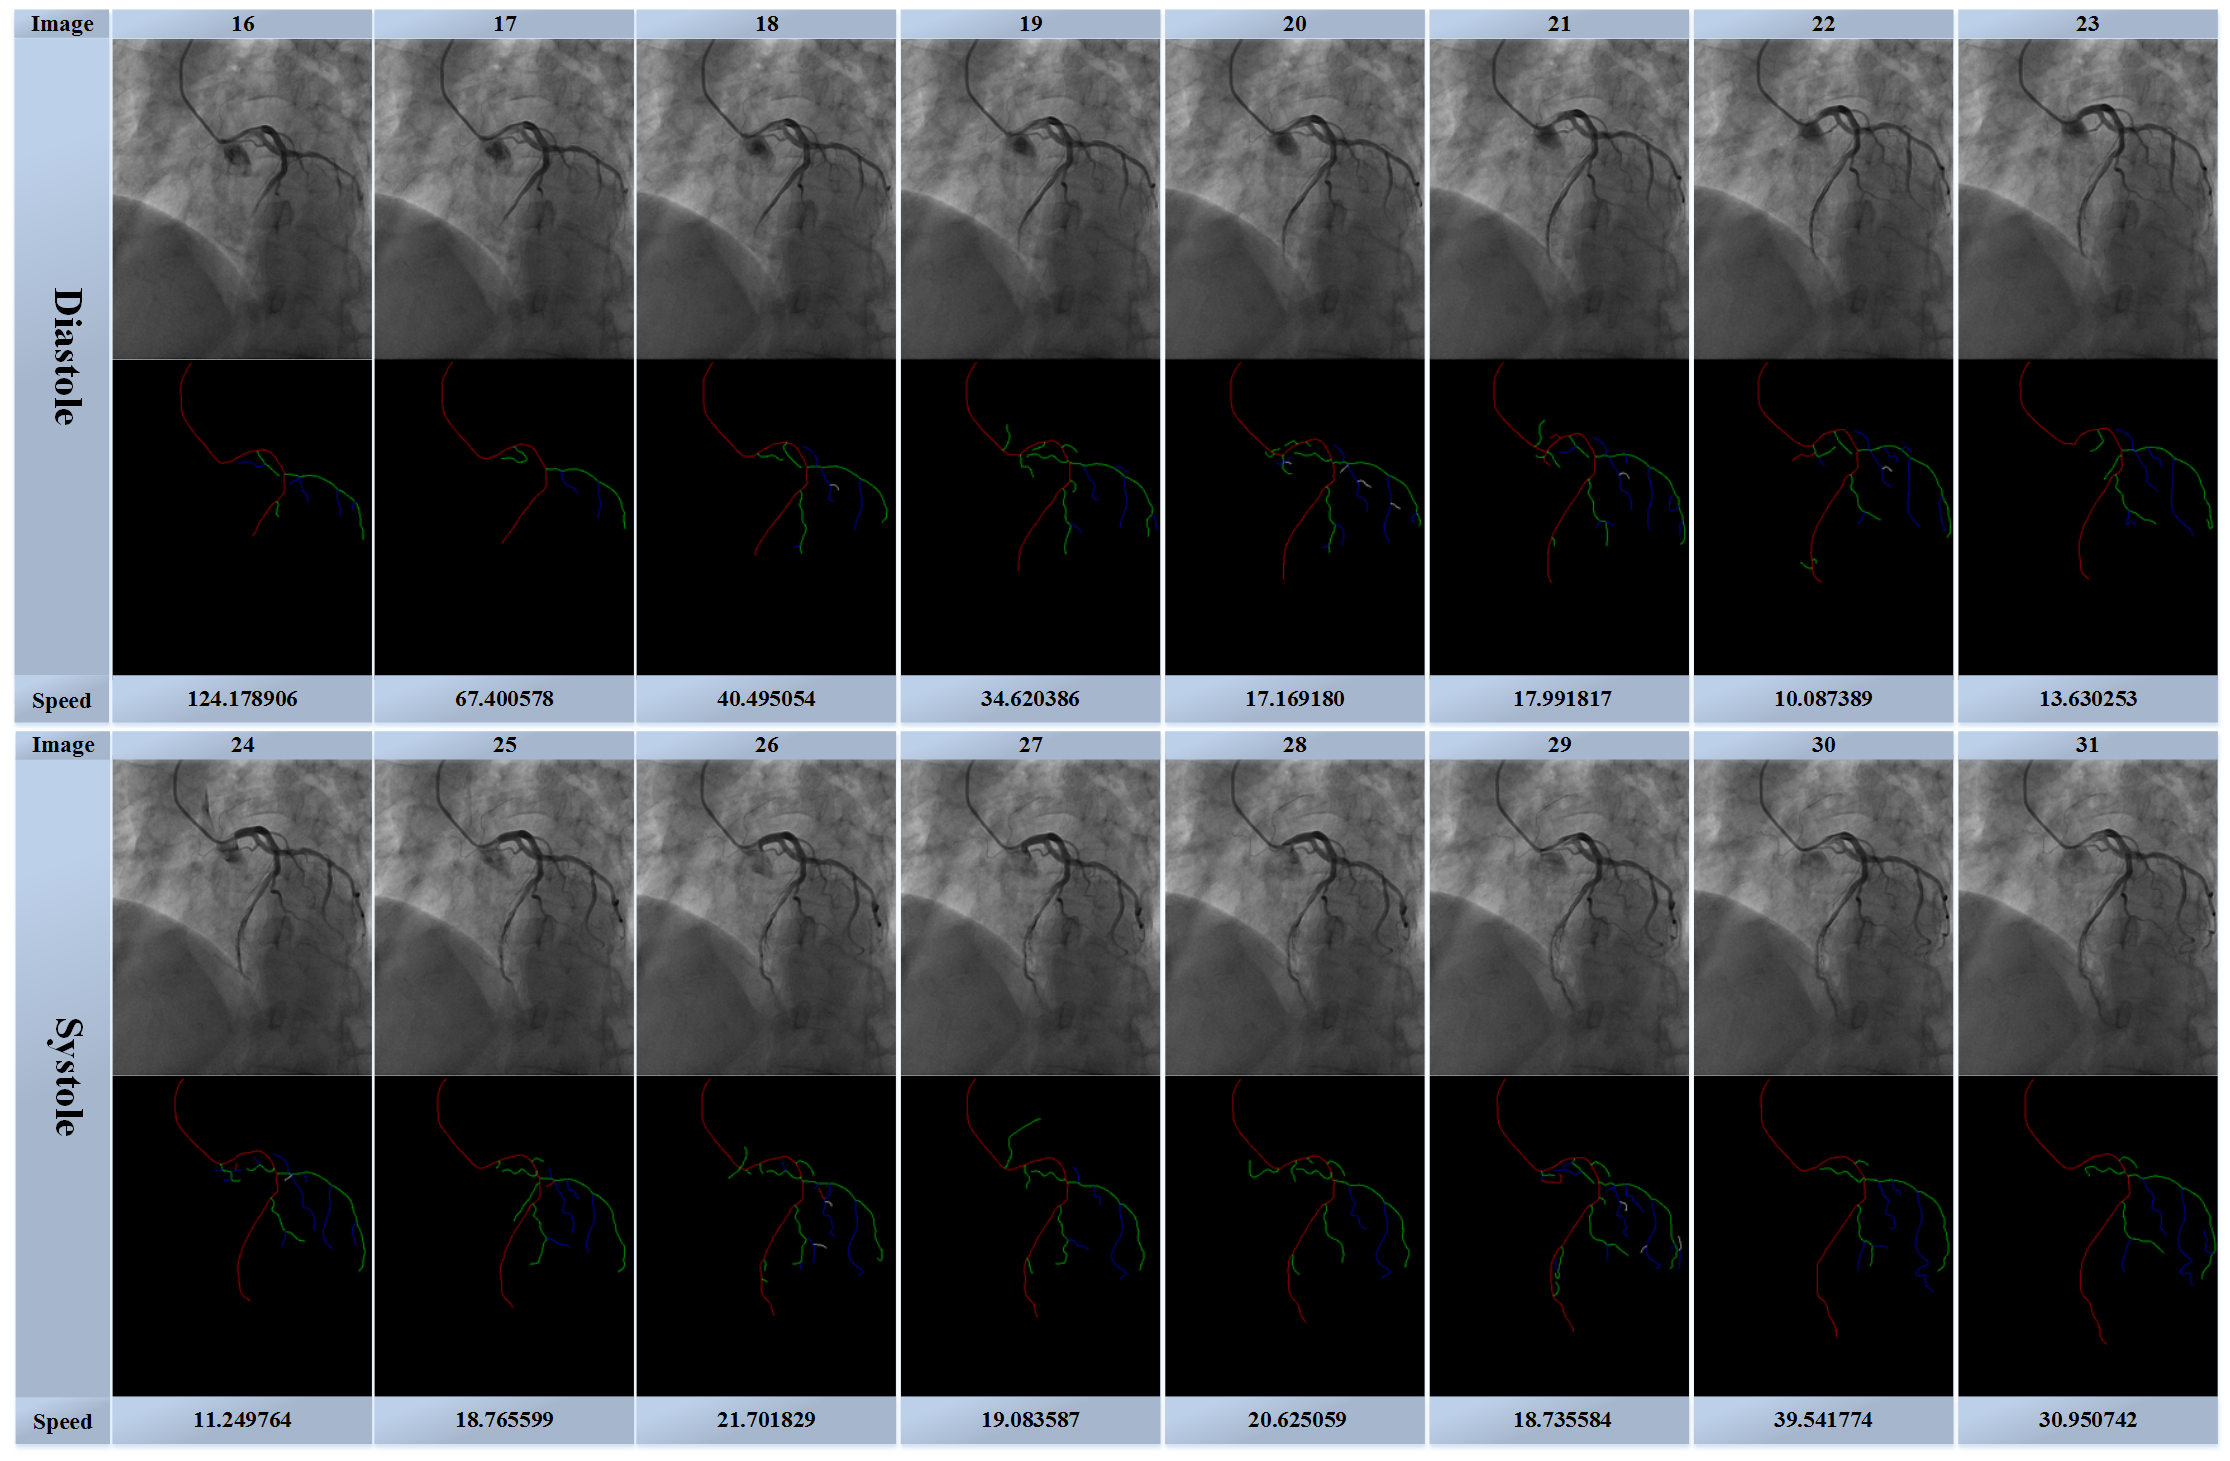
\includegraphics[width=1.0\linewidth]{./images/cardiac_cycle.png}
\caption{One full cardiac cycle with index and velocity.}
\label{fig:app_cardiac_cycle}
\end{figure*}

%%%%%%%%%%%%%%%%%%%%%%%%%%%%%%%%%%%%%%%%%%%%
\section{Experiments and Validation}
\subsection{Tree Organization}
Subsection text here.

\subsection{Vessel Labeling}

\subsection{Application}



% An example of a floating figure using the graphicx package.
% Note that \label must occur AFTER (or within) \caption.
% For figures, \caption should occur after the \includegraphics.
% Note that IEEEtran v1.7 and later has special internal code that
% is designed to preserve the operation of \label within \caption
% even when the captionsoff option is in effect. However, because
% of issues like this, it may be the safest practice to put all your
% \label just after \caption rather than within \caption{}.
%
% Reminder: the "draftcls" or "draftclsnofoot", not "draft", class
% option should be used if it is desired that the figures are to be
% displayed while in draft mode.
%
%\begin{figure}[!t]
%\centering
%\includegraphics[width=2.5in]{myfigure}
% where an .eps filename suffix will be assumed under latex,
% and a .pdf suffix will be assumed for pdflatex; or what has been declared
% via \DeclareGraphicsExtensions.
%\caption{Simulation Results.}
%\label{fig_sim}
%\end{figure}

% Note that IEEE typically puts floats only at the top, even when this
% results in a large percentage of a column being occupied by floats.


% An example of a double column floating figure using two subfigures.
% (The subfig.sty package must be loaded for this to work.)
% The subfigure \label commands are set within each subfloat command,
% and the \label for the overall figure must come after \caption.
% \hfil is used as a separator to get equal spacing.
% Watch out that the combined width of all the subfigures on a
% line do not exceed the text width or a line break will occur.
%
%\begin{figure*}[!t]
%\centering
%\subfloat[Case I]{\includegraphics[width=2.5in]{box}%
%\label{fig_first_case}}
%\hfil
%\subfloat[Case II]{\includegraphics[width=2.5in]{box}%
%\label{fig_second_case}}
%\caption{Simulation results.}
%\label{fig_sim}
%\end{figure*}
%
% Note that often IEEE papers with subfigures do not employ subfigure
% captions (using the optional argument to \subfloat[]), but instead will
% reference/describe all of them (a), (b), etc., within the main caption.


% An example of a floating table. Note that, for IEEE style tables, the
% \caption command should come BEFORE the table. Table text will default to
% \footnotesize as IEEE normally uses this smaller font for tables.
% The \label must come after \caption as always.
%
%\begin{table}[!t]
%% increase table row spacing, adjust to taste
%\renewcommand{\arraystretch}{1.3}
% if using array.sty, it might be a good idea to tweak the value of
% \extrarowheight as needed to properly center the text within the cells
%\caption{An Example of a Table}
%\label{table_example}
%\centering
%% Some packages, such as MDW tools, offer better commands for making tables
%% than the plain LaTeX2e tabular which is used here.
%\begin{tabular}{|c||c|}
%\hline
%One & Two\\
%\hline
%Three & Four\\
%\hline
%\end{tabular}
%\end{table}


% Note that IEEE does not put floats in the very first column - or typically
% anywhere on the first page for that matter. Also, in-text middle ("here")
% positioning is not used. Most IEEE journals use top floats exclusively.
% Note that, LaTeX2e, unlike IEEE journals, places footnotes above bottom
% floats. This can be corrected via the \fnbelowfloat command of the
% stfloats package.



\section{Conclusion}
We have developed a new 4D dynamic vessel reconstruction system from
X-ray angiograms. The uniqueness of our system is its simultaneous
handling on structure, shape, and motion during vessel reconstruction.
The technical core of our system are the parallel algorithms towards
interactive performance. Specifically, at the vessel skeleton
extraction stage, we developed an efficient parallel method to extract
vessels as well as their skeleton and topology from X-ray views. At
the reconstruction stage, we formulate the dynamic reconstruction
problem as an energy optimization problem solved by belief propagation
without explicit registration. The experimental results from both
synthetic and clinical data have shown that our method is robust for
noise and even incomplete data because of the algorithms' global
optimization nature. Our immediate goal for ongoing work is to
continue to improve our system and its functionalities towards clinic
trial in the near future.

% if have a single appendix:
%\appendix[Proof of the Zonklar Equations]
% or
%\appendix  % for no appendix heading
% do not use \section anymore after \appendix, only \section*
% is possibly needed

% use appendices with more than one appendix
% then use \section to start each appendix
% you must declare a \section before using any
% \subsection or using \label (\appendices by itself
% starts a section numbered zero.)
%
%
%
%\appendices
%\section{Proof of the First Zonklar Equation}
%Appendix one text goes here.
%
%% you can choose not to have a title for an appendix
%% if you want by leaving the argument blank
%\section{}
%Appendix two text goes here.


% use section* for acknowledgement
\section*{Acknowledgment}
This work is supported in part by National Natural Science Foundation of China (Grant No. 61190120, 61190121, 61190125, 61300068, 61300067), National Science Foundation of USA (Grant No. IIS-0949467, IIS-1047715, and IIS-1049448), the National High Technology Research and Development Program(863 Program) of China (Grant No. 012AA011503), Postdoctoral Science Foundation of China (Grant No. 2013M530512).


% Can use something like this to put references on a page
% by themselves when using endfloat and the captionsoff option.
\ifCLASSOPTIONcaptionsoff
  \newpage
\fi



% trigger a \newpage just before the given reference
% number - used to balance the columns on the last page
% adjust value as needed - may need to be readjusted if
% the document is modified later
%\IEEEtriggeratref{8}
% The "triggered" command can be changed if desired:
%\IEEEtriggercmd{\enlargethispage{-5in}}

% references section

% can use a bibliography generated by BibTeX as a .bbl file
% BibTeX documentation can be easily obtained at:
% http://www.ctan.org/tex-archive/biblio/bibtex/contrib/doc/
% The IEEEtran BibTeX style support page is at:
% http://www.michaelshell.org/tex/ieeetran/bibtex/
\bibliographystyle{IEEEtran}
\bibliography{bare_jrnl}

% biography section
%
% If you have an EPS/PDF photo (graphicx package needed) extra braces are
% needed around the contents of the optional argument to biography to prevent
% the LaTeX parser from getting confused when it sees the complicated
% \includegraphics command within an optional argument. (You could create
% your own custom macro containing the \includegraphics command to make things
% simpler here.)
%\begin{IEEEbiography}[{\includegraphics[width=1in,height=1.25in,clip,keepaspectratio]{mshell}}]{Michael Shell}
% or if you just want to reserve a space for a photo:

\begin{IEEEbiography}{Xinglong Liu}
Biography text here.
\end{IEEEbiography}

% if you will not have a photo at all:
\begin{IEEEbiographynophoto}{Fei Hou}
Biography text here.
\end{IEEEbiographynophoto}

% insert where needed to balance the two columns on the last page with
% biographies
%\newpage

\begin{IEEEbiographynophoto}{Aimin Hao}
Biography text here.
\end{IEEEbiographynophoto}

\begin{IEEEbiographynophoto}{Hong Qin}
Biography text here.
\end{IEEEbiographynophoto}

% You can push biographies down or up by placing
% a \vfill before or after them. The appropriate
% use of \vfill depends on what kind of text is
% on the last page and whether or not the columns
% are being equalized.

%\vfill

% Can be used to pull up biographies so that the bottom of the last one
% is flush with the other column.
%\enlargethispage{-5in}



% that's all folks
\end{document}


